\documentclass[twoside,11pt]{article}

% ? Specify used packages
\usepackage{graphicx}        %  Use this one for final production.
% \usepackage[draft]{graphicx} %  Use this one for drafting.
\usepackage{array}
\usepackage{fancyhdr}
\usepackage{multirow}
\usepackage{longtable}
\usepackage{color}
\usepackage{caption}
\usepackage{titlesec}
\usepackage{enumitem}
% ? End of specify used packages
\pagestyle{myheadings}
\listfiles
% -----------------------------------------------------------------------------

% ? Document identification
\newcommand{\stardoccategory}  {Starlink Cookbook}
\newcommand{\stardocinitials}  {SC}
\newcommand{\stardocsource}    {sc\stardocnumber}
\newcommand{\stardoccopyright} {Copyright \copyright\ 2014 Science and Technology Facilities Council}
\newcommand{\stardocnumber}    {20.0}
\newcommand{\stardocauthors}   {H.\ S.\ Thomas}
\newcommand{\stardocdate}      {1 September 2014}
\newcommand{\stardoctitle}     {The Heterodyne Data Reduction Cookbook}
\newcommand{\stardocversion}   {1.1}
\newcommand{\stardocmanual}    {\ }
\newcommand{\stardocabstract}  {

   This cookbook provides a short introduction to Starlink facilities,
   especially \textsc{Smurf}, the Sub-Millimetre User Reduction
   Facility and \textsc{Kappa}, the Kernel Application Package, for reducing, displaying, 
   and analysing ACSIS data.
   In particular, this cookbook illustrates the various steps required to reduce the data;
   and gives an overview of the ORAC-DR pipeline which carries out many of these 
   steps using a single command. Specialised pipeline recipes are discussed.}

% ? End of document identification

% -----------------------------------------------------------------------------

% +
%  Name:
%     sc.tex
%
%  Purpose:
%     Template for Starlink Cookbook (SC) documents.
%     Refer to SUN/199
%
%  Authors:
%     AJC: A.J.Chipperfield (Starlink, RAL)
%     BLY: M.J.Bly (Starlink, RAL)
%     PWD: Peter W. Draper (Starlink, Durham University)
%
%  History:
%     16-JUN-1997 (BLY):
%        Original, based on SUN/SG templates.
%     13-AUG-1998 (PWD):
%        Converted for use with LaTeX2HTML version 98.2 and
%        Star2HTML version 1.3.
%      1-FEB-2000 (AJC):
%        Add Copyright statement in LaTeX
%     {Add further history here}
%
% -

\newcommand{\stardocname}{\stardocinitials /\stardocnumber}
\markboth{\stardocname}{\stardocname}
\setlength{\textwidth}{160mm}
\setlength{\textheight}{230mm}
\setlength{\topmargin}{-2mm}
\setlength{\oddsidemargin}{0mm}
\setlength{\evensidemargin}{0mm}
\setlength{\parindent}{0mm}
\setlength{\parskip}{\medskipamount}
\setlength{\unitlength}{1mm}

% -----------------------------------------------------------------------------
%  Hypertext definitions.
%  ======================
%  These are used by the LaTeX2HTML translator in conjunction with star2html.

%  Comment.sty: version 2.0, 19 June 1992
%  Selectively in/exclude pieces of text.
%
%  Author
%    Victor Eijkhout                                      <eijkhout@cs.utk.edu>
%    Department of Computer Science
%    University Tennessee at Knoxville
%    104 Ayres Hall
%    Knoxville, TN 37996
%    USA

%  Do not remove the %begin{latexonly} and %end{latexonly} lines (used by
%  LaTeX2HTML to signify text it shouldn't process).
%begin{latexonly}
\makeatletter
\def\makeinnocent#1{\catcode`#1=12 }
\def\csarg#1#2{\expandafter#1\csname#2\endcsname}

\def\ThrowAwayComment#1{\begingroup
    \def\CurrentComment{#1}%
    \let\do\makeinnocent \dospecials
    \makeinnocent\^^L% and whatever other special cases
    \endlinechar`\^^M \catcode`\^^M=12 \xComment}
{\catcode`\^^M=12 \endlinechar=-1 %
 \gdef\xComment#1^^M{\def\test{#1}
      \csarg\ifx{PlainEnd\CurrentComment Test}\test
          \let\html@next\endgroup
      \else \csarg\ifx{LaLaEnd\CurrentComment Test}\test
            \edef\html@next{\endgroup\noexpand\end{\CurrentComment}}
      \else \let\html@next\xComment
      \fi \fi \html@next}
}
\makeatother

\def\includecomment
 #1{\expandafter\def\csname#1\endcsname{}%
    \expandafter\def\csname end#1\endcsname{}}
\def\excludecomment
 #1{\expandafter\def\csname#1\endcsname{\ThrowAwayComment{#1}}%
    {\escapechar=-1\relax
     \csarg\xdef{PlainEnd#1Test}{\string\\end#1}%
     \csarg\xdef{LaLaEnd#1Test}{\string\\end\string\{#1\string\}}%
    }}

%  Define environments that ignore their contents.
\excludecomment{comment}
\excludecomment{rawhtml}
\excludecomment{htmlonly}

%  Hypertext commands etc. This is a condensed version of the html.sty
%  file supplied with LaTeX2HTML by: Nikos Drakos <nikos@cbl.leeds.ac.uk> &
%  Jelle van Zeijl <jvzeijl@isou17.estec.esa.nl>. The LaTeX2HTML documentation
%  should be consulted about all commands (and the environments defined above)
%  except \xref and \xlabel which are Starlink specific.

\newcommand{\htmladdnormallinkfoot}[2]{#1\footnote{#2}}
\newcommand{\htmladdnormallink}[2]{#1}
\newcommand{\htmladdimg}[1]{}
\newcommand{\hyperref}[4]{#2\ref{#4}#3}
\newcommand{\htmlref}[2]{#1}
\newcommand{\htmlimage}[1]{}
\newcommand{\htmladdtonavigation}[1]{}

\newenvironment{latexonly}{}{}
\newcommand{\latex}[1]{#1}
\newcommand{\html}[1]{}
\newcommand{\latexhtml}[2]{#1}
\newcommand{\HTMLcode}[2][]{}

%  Starlink cross-references and labels.
\newcommand{\xref}[3]{#1}
\newcommand{\xlabel}[1]{}

%  LaTeX2HTML symbol.
\newcommand{\latextohtml}{\LaTeX2\texttt{HTML}}

%  Define command to re-centre underscore for Latex and leave as normal
%  for HTML (severe problems with \_ in tabbing environments and \_\_
%  generally otherwise).
\renewcommand{\_}{\texttt{\symbol{95}}}

% -----------------------------------------------------------------------------
%  Debugging.
%  =========
%  Remove % on the following to debug links in the HTML version using Latex.

% \newcommand{\hotlink}[2]{\fbox{\begin{tabular}[t]{@{}c@{}}#1\\\hline{\footnotesize #2}\end{tabular}}}
% \renewcommand{\htmladdnormallinkfoot}[2]{\hotlink{#1}{#2}}
% \renewcommand{\htmladdnormallink}[2]{\hotlink{#1}{#2}}
% \renewcommand{\hyperref}[4]{\hotlink{#1}{\S\ref{#4}}}
% \renewcommand{\htmlref}[2]{\hotlink{#1}{\S\ref{#2}}}
% \renewcommand{\xref}[3]{\hotlink{#1}{#2 -- #3}}
%end{latexonly}

% -----------------------------------------------------------------------------
% ? Document specific \newcommand or \newenvironment commands.

% Include special HTML versions of commands.

\newcommand{\eg}{{\it e.g.}}
\newcommand{\ie}{{\it i.e.}}

\newsavebox{\fmbox}

% set up description list environment called 'sldes' which has a label taking up 15% of the space on the left - thanks to Sarah Graves for the suggestion.
%\newlist{sldes}{description}{2}
%\setlist[sldes,1,2]{style=nextline, leftmargin=15\textwidth}

%  For the TIP boxes.
\newenvironment{fmpage}[1]{\begin{lrbox}{\fmbox}\begin{minipage}{#1}}{\end{minipage}\end{lrbox}\fbox{\usebox{\fmbox}}}

%  Define additional colours.
\definecolor{gray}{RGB}{200,200,200}
\definecolor{MidnightBlue}{rgb}{0.1, 0.1, 0.44}
\definecolor{bblue}{RGB}{172,207,230}

%  A new environment for quoting verbatim
%  Environment for indenting and using a small font.
\newenvironment{myquote}{
   \color{MidnightBlue}\begin{quote}\begin{small}}{
   \end{small}\end{quote}
}

%\renewcommand{\familydefault}{\sfdefault}

%  This is for coloured banners in section titles.
\newcommand{\colorsection}[1]{%
  \colorbox{bblue}{\parbox{\dimexpr\textwidth-2\fboxsep}{\vspace{0.02cm}\hspace{0.01cm}\thesubsection\vspace{0.01cm}\hspace{0.4cm} #1}}}

\titleformat{name=\subsection}[block]
  {\rmfamily\Large\bfseries}
  {}
  {0pt}
  {\colorsection}
\titlespacing*{\subsection}{0pt}{20pt}{\baselineskip}


%  Shortcuts
%  ---------

% Typographical shortcuts
\newcommand{\fcfbe}{$\mathrm{FCF_{beamequiv}}$}
\newcommand{\fcfb}{$\mathrm{FCF_{beam}}$}
\newcommand{\fcfa}{$\mathrm{FCF_{arcsec}}$}
\newcommand{\fcfm}{$\mathrm{FCF_{match}}$}

% SCUBA reference
%\newcommand{\scuba}{\htmladdnormallink{SCUBA}{http://www.jach.hawaii.edu/JCMT/}}

% Starlink Package name
\newcommand{\starlink}{\htmladdnormallink{Starlink}{http://starlink.jach.hawaii.edu}}

% Set up some common package names.
\newcommand{\ccdpack}{\xref{\textsc{Ccdpack}}{sun139}{}}
\newcommand{\convert}{\xref{\textsc{Convert}}{sun55}{}}
\newcommand{\cupid}{\xref{\textsc{Cupid}}{sun255}{}}
\newcommand{\Figaro}{\xref{\textsc{Figaro}}{sun86}{}}
\newcommand{\fluxes}{\xref{\textsc{Fluxes}}{sun213}{}}
\newcommand{\gaia}{\xref{\textsc{Gaia}}{sun214}{}}
\newcommand{\Kappa}{\xref{\textsc{Kappa}}{sun95}{}}
\newcommand{\agi}{\xref{AGI}{sun48}{}}
\newcommand{\ndf}{\xref{NDF}{sun33}{}}
\newcommand{\surf}{\xref{\textsc{Surf}}{sun216}{}}
\newcommand{\jcmtdr}{\xref{\textsc{JCMTdr}}{sun132}{}}
\newcommand{\oracdr}{\htmladdnormallink{\textsc{Orac-dr}}{http://www.oracdr.org/oracdr}}
\newcommand{\photom}{\xref{\textsc{Photom}}{sun45}{}}
\newcommand{\picard}{\xref{\textsc{Picard}}{sun265}{}}
\newcommand{\smurf}{\xref{\textsc{Smurf}}{sun258}{}}
\newcommand{\splat}{\xref{\textsc{Splat}}{sun243}{}}
\newcommand{\ssds}{\xref{\textsc{Starlink Standard Data Structures}}{sgp38}{}}
\newcommand{\topcat}{\htmladdnormallink{\textsc{Topcat}}{http://www.starlink.ac.uk/topcat}}

% DR recipe names
\newcommand{\drrecipe}[1]{\texttt{#1}}

% Application tasks
\newcommand{\task}[1]{\textsf{#1}}

% ADAM parameters
\newcommand{\param}[1]{\texttt{#1}}

% Environment variables, filenames, URLs, and model names
% These are the same at the moment but could be adjusted in one place.
\newcommand{\envvar}[1]{\texttt{#1}}
\newcommand{\file}[1]{\texttt{#1}}
\newcommand{\model}[1]{\texttt{#1}}
\newcommand{\url}[1]{\texttt{#1}}

% GAIA menu functions and buttons.  Would like a bold texttt to mimic
% their appearance in GAIA, but the founts are not in regular LaTeX.
\newcommand{\gaiathing}[1]{\textbf{\textsf{#1}}}

% SMURF tasks
\newcommand{\jcmtstate}{\xref{\task{jcmtstate2cat}}{sun258}{JCMTSTATE2CAT}}
\newcommand{\makecube}{\xref{\task{makecube}}{sun258}{MAKECUBE}}
\newcommand{\unmakecube}{\xref{\task{unmakecube}}{sun258}{UNMAKECUBE}}


% KAPPA
\newcommand{\beamfit}{\xref{\task{beamfit}}{sun95}{BEAMFIT}}
\newcommand{\cmult}{\xref{\task{cmult}}{sun95}{CMULT}}
\newcommand{\fitslist}{\xref{\task{fitslist}}{sun95}{FITSLIST}}
\newcommand{\chpix}{\xref{\task{chpix}}{sun95}{CHPIX}}
\newcommand{\fitsval}{\xref{\task{fitsval}}{sun95}{FITSVAL}}
\newcommand{\hislist}{\xref{\task{hislist}}{sun95}{HISLIST}}
\newcommand{\histat}{\xref{\task{histat}}{sun95}{HISTAT}}
\newcommand{\block}{\xref{\task{block}}{sun95}{BLOCK}}
\newcommand{\chanmap}{\xref{\task{chanmap}}{sun95}{CHANMAP}}
\newcommand{\clinplot}{\xref{\task{clinplot}}{sun95}{CLINPLOT}}
\newcommand{\collapse}{\xref{\task{collapse}}{sun95}{COLLAPSE}}
\newcommand{\contour}{\xref{\task{contour}}{sun95}{CONTOUR}}
\newcommand{\display}{\xref{\task{display}}{sun95}{DISPLAY}}
\newcommand{\fillbad}{\xref{\task{fillbad}}{sun95}{FILLBAD}}
\newcommand{\gausmooth}{\xref{\task{gausmooth}}{sun95}{GAUSMOOTH}}
\newcommand{\gdstate}{\xref{\task{gdstate}}{sun95}{GDSTATE}}
\newcommand{\linplot}{\xref{\task{linplot}}{sun95}{LINPLOT}}
\newcommand{\mfittrend}{\xref{\task{mfittrend}}{sun95}{MFITTREND}}
\newcommand{\nomagic}{\xref{\task{nomagic}}{sun95}{NOMAGIC}}
\newcommand{\histogram}{\xref{\task{histogram}}{sun95}{HISTOGRAM}}
\newcommand{\lutedit}{\xref{\task{lutedit}}{sun95}{LUTEDIT}}
\newcommand{\makesnr}{\xref{\task{makesnr}}{sun95}{MAKESNR}}
\newcommand{\fittrend}{\xref{\task{mfittrend}}{sun95}{MFITTREND}}
\newcommand{\ndfcopy}{\xref{\task{ndfcopy}}{sun95}{NDFCOPY}}
\newcommand{\ndftrace}{\xref{\task{ndftrace}}{sun95}{NDFTRACE}}
\newcommand{\parget}{\xref{\task{parget}}{sun95}{PARGET}}
\newcommand{\paste}{\xref{\task{paste}}{sun95}{PASTE}}
\newcommand{\provshow}{\xref{\task{provshow}}{sun95}{PROVSHOW}}
\newcommand{\setvar}{\xref{\task{setvar}}{sun95}{SETVAR}}
\newcommand{\stats}{\xref{\task{stats}}{sun95}{STATS}}
\newcommand{\sqorst}{\xref{\task{sqorst}}{sun95}{SQORST}}
\newcommand{\sub}{\xref{\task{sub}}{sun95}{SUB}}
\newcommand{\wcsframe}{\xref{\task{wcsframe}}{sun95}{WCSFRAME}}
\newcommand{\wcsattrib}{\xref{\task{wcsattrib}}{sun95}{WCSATTRIB}}
\newcommand{\wcsmosaic}{\xref{\task{wcsmosaic}}{sun95}{WCSMOSAIC}}
\newcommand{\wcsalign}{\xref{\task{wcsalign}}{sun95}{WCSALIGN}}

% CCDPACK
\newcommand{\makemos}{\xref{\task{makemos}}{sun139}{MAKEMOS}}

% CUPID
\newcommand{\findback}{\xref{\task{findback}}{sun255}{FINDBACK}}
\newcommand{\findclumps}{\xref{\task{findclumps}}{sun255}{FINDCLUMPS}}

% Misc
\newcommand{\autophotom}{\xref{\task{autophotom}}{sun45}{AUTOPHOTOM}}
\newcommand{\fitstondf}{\xref{\task{fits2ndf}}{sun55}{FITS2NDF}}
\newcommand{\hdstrace}{\xref{\task{hdstrace}}{sun95}{HDSTRACE}}

% Documents
\newcommand{\gaiasun}{\xref{\textbf{SUN/214}}{sun214}{}}
\newcommand{\ccdpacksun}{\xref{\textbf{SUN/139}}{sun139}{}}
\newcommand{\kappasun}{\xref{\textbf{SUN/95}}{sun95}{}}
\newcommand{\picardsun}{\xref{\textbf{SUN/265}}{sun265}{}}
\newcommand{\pipelinesun}{\xref{\textbf{SUN/260}}{sun264}{}}
\newcommand{\smurfsun}{\xref{\textbf{SUN/258}}{sun258}{}}
\newcommand{\convertsun}{\xref{\textbf{SUN/55}}{sun55}{}}
\newcommand{\cupidsun}{\xref{\textbf{SUN/255}}{sun255}{}}
\newcommand{\oracdrsun}{\xref{\textbf{SUN/230}}{sun230}{}}
\newcommand{\hdstracesun}{\xref{\textbf{SUN/102}}{sun102}{}}
\newcommand{\gaiasc}{\xref{\textbf{SC/17}}{sc17}{}}
\newcommand{\splatsun}{\xref{\textbf{SUN/243}}{sun243}{}}

% Chapter title in the header. This is using package fancyhdr.
\pagestyle{fancy}
\renewcommand{\sectionmark}[1]{\markboth{\stardocname---#1}{\stardocname---#1}}
\renewcommand{\subsectionmark}[1]{}
\renewcommand{\headrulewidth}{0pt}
\lhead{\thepage}
\fancyfoot[c]{}
\fancyfoot[r]{}

% Figure environment. Defined for latex2html to produce good quality
% graphics in the hypertext. It assumes that the files are
% encapsulated PostScript with extension .eps, and PNG with extension
% .png. The arguments are: #1 graphics filename without an extension;
% #2 figure environment location including brackets, or leave empty for
% none; #3 the includegraphics % qualifiers; #4 the label; #5 is the
% short caption for the index of figures; and #6 is the full caption.
\newcommand{\myfig}[6]{
  \begin{figure}#2
    \centering\includegraphics[#3]{#1}
    \typeout{#1 inserted on page \arabic{page}}
    \caption[#5]{\label{#4}\small #6}
  \end{figure}
}
\begin{htmlonly}
  \newcommand{\myfig}[6]{
    \label{#4} \htmladdimg{#1.png}\\
    \\
    Figure: #6\\
  }
\end{htmlonly}

% Address twin (side-by-side) graphics in a similar fashion where the
% second argument is the second graphic, and the remaining arguments
% incremented by one slot save an extra argument #6 for the size of
% the gap between the two graphics, thus #7 and #8 are the captions.
\newcommand{\myfigduo}[8]{
  \begin{figure}#3
    \includegraphics[#4]{#1}
    \typeout{#1 inserted on page \arabic{page}}
    \hspace{#6}
    \includegraphics[#4]{#2}
    \typeout{#2 inserted on page \arabic{page}}
    \caption[#7]{\label{#5}\small #8}
  \end{figure}
}
\begin{htmlonly}
  \newcommand{\myfigduo}[8]{
    \label{#5} \htmladdimg{#1.png}\htmladdimg{#2.png}\\
    \\
    Figure: #8\\
  }
\end{htmlonly}

% A command to cross-reference in both LaTeX and hypertext.
% #1 is the type such as Section, Table, Figure; #2 is
% the label; and #3 is the text or title associated with the
% reference.
\newcommand{\cref}[3]{\latexhtml{#1~\ref{#2}}{\htmlref{#3}{#2}}}

%  LaTex2HTML has a problem with coloured text swapping it from
%  the \myquote context to the main text.

\begin{htmlonly}
   \renewenvironment{myquote}{
      \begin{quote}\begin{small}}{
      \end{small}\end{quote}
   }
\end{htmlonly}


% ? End of document specific commands
% -----------------------------------------------------------------------------
%  Title Page
%  ==========
\renewcommand{\thepage}{\roman{page}}
\begin{document}
\thispagestyle{empty}

%  Latex document header
%  =====================
\begin{latexonly}
   \textsc{Joint Astronomy Centre} \hfill \textbf{\stardocname}\\
   {\large Science \& Technology Facilities Council}\\
   {\large Starlink Project\\}
   {\large \stardoccategory\ \stardocnumber}
   \begin{flushright}
   \stardocauthors\\
   \stardocdate
   \end{flushright}
   \vspace{-4mm}
   \rule{\textwidth}{0.5mm}
   \vspace{5mm}
   \begin{center}
   {\Huge\textbf{\stardoctitle \\ [2.5ex]}}
   {\LARGE\textbf{\stardocversion \\ [4ex]}}
   {\Huge\textbf{\stardocmanual}}
   \end{center}
   \vspace{5mm}

% ? Add picture here if required for the LaTeX version.
%   e.g. \includegraphics[scale=0.3]{filename.ps}
% ? End of picture
   \begin{center}
%   \includegraphics[scale=0.4]{sc21_s2logo}
   \end{center}
   \vspace{5mm}
   \rule{\textwidth}{0.5mm}\\
   \vspace{15mm}

% ? Heading for abstract if used.
   \vspace{10mm}
   \begin{center}
      {\Large\textbf{Abstract}}
   \end{center}
% ? End of heading for abstract.

\end{latexonly}

%  HTML documentation header
%  =========================
\begin{htmlonly}
   \xlabel{}
   \begin{rawhtml} <H1> \end{rawhtml}
      \stardoctitle\\
      \stardocversion\\
      \stardocmanual
   \begin{rawhtml} </H1> <HR> \end{rawhtml}

% ? Add picture here if required for the hypertext version.
%   e.g. \includegraphics[scale=0.5]{filename.ps}
%   \includegraphics[width=90mm]{sc21_s2logo}
% ? End of picture

   \begin{rawhtml} <P> <I> \end{rawhtml}
   \stardoccategory\ \stardocnumber \\
   \stardocauthors \\
   \stardocdate
   \begin{rawhtml} </I> </P> <H3> \end{rawhtml}
      \htmladdnormallink{Joint Astronomy Centre}
                        {http://www.jach.hawaii.edu}\\
      \htmladdnormallink{Science \& Technology Facilities Council}
                        {http://www.scitech.ac.uk} \\
   \begin{rawhtml} </H3> <H2> \end{rawhtml}
      \htmladdnormallink{Starlink Project}{http://www.starlink.ac.uk/}
   \begin{rawhtml} </H2> \end{rawhtml}
   \htmladdnormallink{\htmladdimg{source.gif} Retrieve hardcopy}
      {http://www.starlink.ac.uk/cgi-bin/hcserver?\stardocsource}\\

%  HTML document table of contents
%  ===============================
%  Add table of contents header and a navigation button to return to this
%  point in the document (this should always go before the abstract \section).
  \label{stardoccontents}
  \begin{rawhtml}
    <HR>
    <H2>Contents</H2>
  \end{rawhtml}
  \htmladdtonavigation{\htmlref{\htmladdimg{contents_motif.gif}}
        {stardoccontents}}

% ? New section for abstract if used.
  \section{\xlabel{abstract}Abstract}
% ? End of new section for abstract
\end{htmlonly}

% -----------------------------------------------------------------------------
%  Document Abstract
%  =================
\stardocabstract
% ? End of document abstract

% -----------------------------------------------------------------------------
%  Latex Copyright Statement
%  =========================
\begin{latexonly}
  \newpage
  \vspace*{\fill}
  \stardoccopyright
\end{latexonly}
% ? End of Latex copyright statement

% -----------------------------------------------------------------------------
%  Latex document Table of Contents
%  ================================
  \newpage
  \begin{latexonly}
    \setlength{\parskip}{0mm}
    \tableofcontents
    \newpage
    \listoffigures
    \setlength{\parskip}{\medskipamount}
    \markboth{\stardocname}{\stardocname}
  \end{latexonly}
% ? End of Latex document table of contents

% -----------------------------------------------------------------------------

%  Glossary
%  ========
\newpage
\begin{latexonly}
\addcontentsline{toc}{section}{Acronyms}
% ? Heading for glossary if used.
   \vspace{10mm}
   \begin{center}
      {\Large\textbf{Acronyms}}
   \end{center}
% ? End of heading for glossary.
\setlength{\extrarowheight}{3pt}
\begin{table}[h!]
\begin{tabular}{ll}

\textbf{ACSIS}& Auto-Correlation Spectrometer and Imaging System\\
\textbf{ARD}& ASCII Region Definition\\
\textbf{CADC}& Canadian Astronomy Data Centre\\
\textbf{CSO}& Caltech Submillimetre Observatory\\
\textbf{FITS}& Flexible Image Transport System\\
\textbf{FWHM}& Full-Width at Half-Maximum\\
\textbf{GAIA}& Graphical Astronomy and Image Analysis Tool\\
\textbf{HDS}& Hierarchical Data System\\
\textbf{JCMT}& James Clerk Maxwell Telescope\\
\textbf{LSB}& Lower sideband\\
\textbf{NDF}& Extensible N-Dimensional Data Format\\
\textbf{HARP}& Heterodyne Array Receiver Programme\\
\textbf{QA}& Quality Assurance\\
\textbf{RxA}& Receiver A\\
\textbf{SDF}& Starlink Data File\\
\textbf{S/N}& Signal-to-Noise ratio\\
\textbf{USB}& Upper sideband\\
\textbf{WVM}& Water Vapour radioMeter\\
\end{tabular}
\end{table}

\end{latexonly}

% -----------------------------------------------------------------------------

\cleardoublepage
\renewcommand{\thepage}{\arabic{page}}
\setcounter{page}{1}

%  This is for chapter-like headings.  It must come after the tables of
%  contents and figures to avoid these having a zero chapter number
%  appearing.  The comments before the \begin{latexonly} and
%  \begin{latexonly} environment must be retained for the definitions
%  to persist outside this block.  See MUD/152, p38.
%  Despite the latexonly environment, this causes the HTML some grief
%  and creates < section headings.
%\begin{latexonly}
  \titleformat{\section}[display]
     {\normalfont\huge\bfseries}
      {}
     {0pt}
     {Chapter \thesection\newline}
     \titlespacing*{\section}{0pt}{0pt}{20pt}
%\end{latexonly}


\section{\xlabel{introduction}Introduction}
\label{sec:intro}

\subsection{\xlabel{using_guide}This cookbook}
This cookbook is designed to instruct ACSIS users on the best ways to
reduce and visualise their data using \starlink\ packages.

This guide covers the following:
\begin{itemize}
\itemsep0em 
\item \cref{Chapter}{sec:intro}{Chapter 1} -- Computer resources you'll need before getting started.
\item \cref{Chapter}{sec:starlink}{Chapter 2} -- Starlink basics -- tools for exploring your data.
\item \cref{Chapter}{sec:het}{Chapter 3}  -- Heterodyne observing at the JCMT.
\item \cref{Chapter}{sec:raw}{Chapter 4}  -- Examining raw ACSIS data.
\item \cref{Chapter}{sec:reduce}{Chapter 5}  -- Regridding your data with \makecube.
\item \cref{Chapter}{sec:analyse}{Chapter 6}  -- Analysing your reduced cube.
\item \cref{Chapter}{sec:advanced}{Chapter 7}  -- Advanced analysis techniques such as changing coordinate frames.
\item \cref{Chapter}{sec:gaia}{Chapter 7}  -- Using \gaia\ to analyse your data.
\item \cref{Chapter}{sec:pipe}{Chapter 8}  -- The ACSIS pipeline and recipes explained.
\item \cref{Chapter}{sec:runpipe}{Chapter 9}  -- How to run the pipeline.
\end{itemize}

\textbf{Style convention}\\
In this cookbook the following styles are followed:
\begin{itemize}[noitemsep,nolistsep]
\item \texttt{\%}  represents the command-line prompt.
\item Command line examples are shown in \texttt{\color{MidnightBlue}{navy typewriter font.}}
\item The names of \gaia\ commands or windows appear in \textbf{bold}. 
\item Useful tips of reminders are given in outlined boxes.
\end{itemize}

\subsection{\xlabel{software}Before you start: Starlink software}

This manual utilises software from the \starlink\ package;
\smurf\ \cite{smurf}, \Kappa\ \cite{kappa}, \gaia\ \cite{gaia}, \oracdr\ \cite{oracdr}, \convert\ \cite{convert}, \ccdpack\ \cite{ccdpack}, and
\picard\ \cite{picard}. Starlink software must be installed on your system, and Starlink aliases
and environment variables must be defined before attempting any ACSIS data reduction. You can download Starlink from \xref{the Starlink webpage}{\starlink}{}.

Below is a brief summary of the packages used in this cookbook and how to initialise them. Note that all the example commands are shown with a UNIX shell. 

\begin{table}[h!]
\begin{tabular}{p{1.7cm}|p{7.4cm}|p{2.9cm}|p{2.2cm}}

\textbf{Package} & \textbf{Description} & \textbf{Initialise}  & \textbf{Help}\\
\hline
\smurf\ & The Sub-Millimetre User Reduction Facility (\smurf) contains \makecube\ that will process raw ACSIS data into spectral cubes. & \texttt{\%\,smurf} & \texttt{\%\,smurfhelp} \newline \smurfsun\\
\hline
\Kappa\ & A general purpose  applications package with commands for processing, visualising, and manipulating NDFs. & \texttt{\%\,kappa} & \texttt{\%\,kaphelp} \newline \kappasun\ \\
\hline
\convert\ &  CONVERT allows the interchange of data files to and from NDF. Other formats include IRAF, FITS, and ASCII. & \texttt{\%\,convert} & \texttt{\%\,conhelp} \newline \convertsun\ \\
\hline
\cupid\ & CUPID is a package of commands that allows the identification and analysis of clumps of emission within 1-, 2- or 3-dimensional data arrays &  \texttt{\%\,cupid} & \texttt{\%\,cupidhelp} \newline \cupidsun\ \\
\hline
\oracdr\ & The \oracdr\ Data Reduction Pipeline \cite{oracdr} is an automated reduction pipeline. \textsc{Orac-dr} uses
\smurf\ and \Kappa\ (along with other Starlink tools) to perform an automated
reduction of the raw data following pre-defined recipes.& \texttt{\%\,oracdr\_acsis} &  \oracdrsun \\
\hline
\textsc{Picard} &  \textsc{Picard} uses a similar pipeline system as \oracdr\ but for the post-processing of reduced data. While mainly implemented for SCUBA-2 data, there are a few recipes that are heterodyne compatible. See \cref{Appendix}{app:picard}{Picard} for more details and a description of available recipes.& \texttt{\%\,picard RECIPE $<$files$>$} & \picardsun\ \\
\hline
\multicolumn{4}{l}{}\\
\textbf{Tool} & \textbf{Description} & \textbf{Open}  & \textbf{Help}\\
\hline
\gaia\ & \gaia\ is an interactive image and data-cube display and analysis tool. It incorporates tools such
as source detection, 3-dimensional visualisation, clump visualisation, photometry and the ability
to query and overlay on-line or local catalogues. & \texttt{\%\,gaia} & \gaiasun\ \gaiasc\ \\
\hline
\splat\ & \splat\ is a graphical spectral-analysis tool. It can also interact with the Virtual Observatory.  & \texttt{\%\,splat}  & \splatsun\ \\
\hline
\end{tabular}
\end{table}

\subsection{\xlabel{software}Options for Reducing you Data}

You have three options for processing your data:
\\\\
(1) Performing each step manually.\\
(2) Write your own scripts, and \\
(3) Running the automated pipeline.
\\\\
The pipeline approach works well if your project is suited to using one of the
standard recipes, and if you have a lot of data to process. Performing
each step by hand allows more fine-tuned control of certain
processing and analysis steps, although some fine tuning is available in the pipeline via recipe parameters (see \cref{Section}{sec:recpars}{Recipe parameters}). 

Once you have determined you optimal parameters you can pass them to the
pipeline or a script. Chapters~5 and 6 discuss the manual approach. To use the science pipeline, skip
straight to \cref{Chapter}{sec:pipe}{The ACSIS Pipeline}.

While you have the option of running the pipeline yourself, you can find pipeline reduced files for individual and coadded observations by night in the \htmladdnormallink{JCMT Science Archive}{http://www3.cadc-ccda.hia-iha.nrc-cnrc.gc.ca/jcmt/} (JSA). These have been reduced using the \oracdr\ pipeline with the recipe specified in the MSB. PIs and co-Is can access this data through the JSA before it becomes public by following the instructions in \cref{Chapter}{sec:runpipe}{The ACSIS Pipeline}.

\newpage
\section{\xlabel{starlink}Good to know: Starlink}
\label{sec:starlink}
\subsection{File format}
\label{sec:format}
Starlink routines run on HDS files (Hierarchical Data System) which normally have a .sdf extension (Starlink Data File). HDS files can describe a multitude of formats. The most common HDS format you will encounter is the NDF (N-Dimensional Data Format). This is the standard file format for storing data which represent N-dimensional arrays of numbers, such as spectra, images, etc. The parameter files discussed in Section \ref{sec:hdstrace} are also HDS format.

Raw data retrieved from the JCMT Science Archive comes in FITS format. For information on converting between FITS and NDF see \cref{Appendix}{app:convert}{Converting file formats}. 

\subsection{\xlabel{adam}How to find the current parameter values}
\label{sec:hdstrace}
A directory called \texttt{adam} is created in your home-space by default when you run Starlink applications. In this directory you will find HDS files for each of the application that you have run. These files contain the parameters used and results returned (if appropriate) from the last time you ran a particular application.

You can specify a different location for the \texttt{adam} directory by setting the environment variable \texttt{ADAM\_USER} to be the path to your alternative location. This is useful when running more than one reduction to avoid interference or access clashes.

To see the ADAM parameters, run \hdstrace\ on any of the parameter files. For example, to see which parameters were used and the results from last time you ran \stats, you can type the following from  anywhere on your system:
{\color{MidnightBlue}\begin{myquote}
\begin{verbatim}
% hdstrace ~/adam/stats
\end{verbatim}
\end{myquote}}
This will report the following
\begin{quote}
\begin{verbatim}
STATS  <STRUC>
   ADAM_DYNDEF    <DEFAULTS>      {structure}
   COMP           <_CHAR*132>     'DATA'
   ORDER          <_LOGICAL>      TRUE
   MAXIMUM        <_DOUBLE>       36.666870117188
   MAXWCS         <_CHAR*132>     '10.625136, -0.381122, -6.057133'
   MINWCS         <_CHAR*132>     '10.720136, -0.017795, -31.05713'
   MEAN           <_DOUBLE>       0.25890738014562
   MINIMUM        <_DOUBLE>       -2.7510244846344
   SIGMA          <_DOUBLE>       0.72429928153974
    ..               ..                 ..
    ..               ..                 ..
\end{verbatim}
\end{quote}
\vspace{0.3cm}
You can see \stats\ was run on the data array with ordered statistics as well as the resulting values. Any of the parameters returned by running \hdstrace\ on an ADAM file can be extracted using the command \task{parget}. In the example below, the mean value from the last instance of \task{stats} is printed to the screen.
{\color{MidnightBlue}\begin{myquote}
\begin{verbatim}
% parget mean stats
\end{verbatim}
\end{myquote}}

 \textbf{Extracting a value for scripting:}\\
\parget\ is designed to make life easier when passing values between shell scripts. In the C-shell scripting example below, the  median value from \task{histat} is assigned to the variable med.
\vspace{0.3cm}

\texttt{set med = \`{}parget median histat\`{}}
\vspace{0.3cm}

If the parameter comprises a vector of values these can be stored in a C-shell array. For other scripting languages such as Python, the alternative vector format produced by setting parameter VECTOR to TRUE may be more appropriate. Single elements of a parameter array may also be accessed using the array index in parentheses.

In addition to running \task{hdstrace} on the ADAM file, you can find a list of all parameter names that can be returned with \parget\ in the \xref{\textsc{Kappa} manual}{sun95}{} under `Results parameters'  for the command in question. Note that these names may be different from the names returned in a terminal when running application.

\subsection{How can I view the metadata?}
\label{sec:fitslist}
There are two \Kappa\ tasks which are extremely useful for examining your metadata: \fitslist\ and \ndftrace, which can be used to view the FITS headers and properties, such as dimensions,  of the data respectively. The third option is the stand-alone application \hdstrace.
\vspace{0.7cm}\\
\begin{minipage}[t]{0.12\linewidth}
\textbf{fitslist}
\end{minipage}
\begin{minipage}[t]{0.85\linewidth}This lists the FITS header information
for any NDF (raw or reduced). This extensive list includes dates \& times,
source name, observation type, band width, number of channels, receptor information, exposure
time, start and end elevation and opacity. In the example below, just the object name is extracted.
{\color{MidnightBlue}\begin{myquote}
\begin{verbatim}
% fitslist file | grep OBJECT
\end{verbatim}
\end{myquote}}
Likewise, if you know the name of the parameter you want to view you can
use the \fitsval\ command instead, e.g.
{\color{MidnightBlue}\begin{myquote}
\begin{verbatim}
% fitsval file OBJECT
\end{verbatim}
\end{myquote}}
\end{minipage}
\vspace{0.7cm}\\
\begin{minipage}[t]{0.12\linewidth}
\textbf{ndftrace}
\end{minipage}
\begin{minipage}[t]{0.85\linewidth}
\task{ndftrace} displays the attributes of the NDF data structure. This will tell you, for example,  the units of the data, pixel bounds, dimensions and axis assignations.
{\color{MidnightBlue}\begin{myquote}
\begin{verbatim}
% ndftrace map fullframe fullwcs

\end{verbatim}
\end{myquote}}
\end{minipage}

\begin{minipage}[t]{0.12\linewidth}
\textbf{hdstrace}
\end{minipage}
\begin{minipage}[t]{0.85\linewidth}
\task{hdstrace} lists the name, data type and values of an HDS (Hierarchical Data System) object. The following example shows the structure of a time-series cube, including the pixel origin of the data structure. To show just the first $x$ lines of values for each parameter include the option \param{nlines=x} on the command line:
{\color{MidnightBlue}\begin{myquote}
\begin{verbatim}
% hdstrace file nlines=3
\end{verbatim}
\end{myquote}}
Otherwise to see all the lines and information that is available in each extension use \param{nlines=all}. The example below displays all the system temperature values and pipes the result to `less' to make viewing easier. 
{\color{MidnightBlue}\begin{myquote}
\begin{verbatim}
% hdstrace file.MORE.ACSIS.TSYS nlines=all | less
\end{verbatim}
\end{myquote}}
\end{minipage}
\vspace{0.4cm}

You can see it descends two levels (into \texttt{MORE} and \texttt{ACSIS}) to retrieve the information. Other information available at this level include receptors and receiver temperatures.

Full details of \ndftrace\ and \fitslist\ can be found in the \xref{\textsc{Kappa} manual}{sun95}{}. Details on \hdstrace\  can be found in the \xref{\textsc{hdstrace} manual}{sun102}{}.

\begin{latexonly}
\begin{center}
\begin{fmpage}{0.95\linewidth}
\vspace{0.1cm}
TIP: The `.sdf' extension on filenames is not required when running Starlink commands.
\end{fmpage}
\end{center}
\end{latexonly}

\begin{htmlonly}
\textbf{TIP: The `.sdf' extension on filenames is not required when running Starlink commands.\\*\\*}
\end{htmlonly}


\subsection{What has already been done to the data?}

If you are presented with a data file you may wish to see what commands have been run on it and, in the case of a coadded cube, which data went into it. Two \Kappa\ commands can help you with this:
\vspace{0.7cm}\\
\begin{minipage}[t]{0.12\linewidth}
\textbf{hislist}
\end{minipage}
\begin{minipage}[t]{0.85\linewidth}The \Kappa\ command \hislist\ will return the history records of the NDF. 
{\color{MidnightBlue}\begin{myquote}
\begin{verbatim}
% hislist myfile brief
\end{verbatim}
\end{myquote}}
Including the \param{brief} option returns a simple list of the commands. Omitting this will include the text associated with each command and can be useful for finding out what parameters were used in each case. This works for all NDFs including those reduced by the pipeline, for these all the commands executed as part of the pipeline reduction script will be listed. The version of software used for each step is also reported.
\end{minipage}
\vspace{0.7cm}\\
\begin{minipage}[t]{0.12\linewidth}
\textbf{provshow}
\end{minipage}
\begin{minipage}[t]{0.85\linewidth}
The \Kappa\ command \task{provshow} displays the details of the NDFs that were used in the creation of the given file. It includes both immediate parents and older ancestor NDFs. 
{\color{MidnightBlue}\begin{myquote}
\begin{verbatim}
% provshow file
\end{verbatim}
\end{myquote}}
\end{minipage}   
\vspace{0.7cm}\\

\subsection{\xlabel{ndfsections}How to examine, process or extract a subset of your data}
\label{sec:ndfsections}
For all Starlink commands you can specify a sub-section of your data on which to run an application. You do this by appending the NDF name with the bounds of the section to be  processed. This may be on the command line or in response to a prompt. 

The example below runs \stats\ on a sub-cube within your original cube. This sub-cube is defined by bounds given for each axis. The upper and lower bounds for each axis are separated by a colon, while the axes themselves are separated by a comma. Note that the use of quotes is necessary on a UNIX shell command line but not in response to a prompt.
{\color{MidnightBlue}\begin{myquote}
\begin{verbatim}
% stats `cube(10.5:10.0,0.0:0.25,-25:25)'
\end{verbatim}
\end{myquote}}
The bounds are given in the coordinates of the data (Galactic for Axes 1 and 2 and velocity for Axis 3). You can find the number and names of the axes along with the pixel bounds of your data file by running \ndftrace. In the example above the ranges are 10.5$^\circ$ to 10$^\circ$ in Longitude (note the range goes from left to right), 0$^\circ$ to 0.25$^\circ$ in Latitude, and -25 to +25 km/s in velocity. In the velocity axes one pixel is one channel. To leave an axis untouched simply include the comma but do not specify any bounds.

To define your bounds in FK5 coordinates use the following format.
{\color{MidnightBlue}\begin{myquote}
\begin{verbatim}
% stats `cube(22h18m:22h32m,05d:05d30m,)'
\end{verbatim}
\end{myquote}}

To write a section of your data into a new file (called newcube in the example below) use \ndfcopy\ with bounds. 
{\color{MidnightBlue}\begin{myquote}
\begin{verbatim}
% ndfcopy `cube(10.5:10.0,0.0:0.25,-25:25)' newcube title="l=10.5 sub-section"
\end{verbatim}
\end{myquote}}
Here the option \param{title} defines a title for the new cube which replaces the title derived from the original.

You can also define a region as a number of pixels from a given origin. The example below extracts a 25$\times$25 pixels cube around the position $l=10^\circ$, $b=0^\circ$.
{\color{MidnightBlue}\begin{myquote}
\begin{verbatim}
% ndfcopy `cube(10.0~25:0.0~25,)' newcube
\end{verbatim}
\end{myquote}}

\begin{latexonly}
\begin{center}
\begin{fmpage}{0.95\linewidth}
\vspace{0.1cm}
TIP: To help identify your sub-region in pixel coordinates, open your file in \gaia\ and change the built-in coordinates to PIXEL via \gaiathing{Image-Analysis} $>$ \gaiathing{Change coordinate} $>$ \gaiathing{Build-in coordinates}. 
\end{fmpage}
\end{center}
\end{latexonly}

\begin{htmlonly}
\textbf{TIP: To help identify your sub-region in pixel coordinates, open your file in \gaia\ and change the built-in coordinates to PIXEL via \gaiathing{Image-Analysis}$>$ \gaiathing{Change coordinate}$>$ \gaiathing{Build-in coordinates}. \\*\\*}
\end{htmlonly}

\newpage
\subsection{\xlabel{help}How to get help}
\label{sec:help}
\begin{table}[h!]
\begin{tabular}{p{2.3cm}|p{7.3cm}|p{5cm}}
\textbf{Command} & \textbf{Description} & \textbf{Usage}\\
\hline
\task{showme} & If you know the name of the Starlink document you want to view
                use \task{showme}. When run, it launches a new web page or tab
                displaying the hypertext version of the document. &
                \texttt{\% showme sun95}\\
\hline
\task{findme} & \task{findme} searches Starlink documents for a keyword. When
                run, it launches a new web page or tab listing the results. &
                \texttt{\% findme kappa} \newline  \texttt{\% findme heterodyne}\\
\hline
\task{docfind} & \task{docfind} searches the internal list files for keywords. It then
                 searches the document titles. The result is displayed using the
                 UNIX \task{more} command. & \texttt{\% docfind kappa}\\
\hline
Run routines with prompts & You can run any routine with the option
                            \texttt{prompt} after the command. This will
                            prompt for every parameter available. If you
                            then want a further description of any parameter
                            type  \texttt{?} at the relevant prompt. &
                            \texttt{\% makemap prompt \newline\ \% REF - Ref. NDF /!/$>$ ?}\\
\hline
\end{tabular}
\end{table}


\clearpage
\section{\xlabel{het_overview}JCMT Heterodyne Observing}
\label{sec:het}
\subsection{\xlabel{specline}Spectral-line Observing}
Submillimetre instruments use heterodyne techniques to observe spectral lines at high resolution. Heterodyne receivers take a weak incoming signal and mix it with a reference frequency known as the local oscillator (LO). This results in a signal of lower (intermediate) frequency (IF) which can be amplified and more easily sampled. JCMT receivers have an IF of 4\,GHz. This mixing produces two frequencies for each value of the LO ($\nu_{sky} = \nu_{LO}\pm\nu_{IF}$) which are known as the upper sideband (USB) and lower sideband (LSB). 

In a single sideband receiver one of these is suppressed. Double sideband receivers have the two frequencies superimposed.

Reducing the noise in the system is crucial to the efficiency of these receivers. The required integration time is directly proportional to the total noise in the system given by $T_{sys}$) via the radiometer formula

\[T_A^*(rms) = \frac{2\,T_{sys}\,\kappa}{\sqrt{\Delta\nu\,t}}\]

where the terms are as follows:
\begin{itemize}
\item $\Delta\nu$ is the frequency resolution of each channel.

\item $t$ is the total integration time (time spent integrating on the source and the reference position).

\item $\kappa$ is the telescope specific backend degradation factor. 

\item The factor of 2 is required for  position-switch or beam-switch observations where half the time is spend off source at the reference position. It may be omitted for frequency switched observations.

\item $T_{sys}$ is the  system temperature in kelvins and describes the total noise of the system. It includes contributions from the background sky temperature, the Earth's atmosphere, ground spillover picked up by the side lobes and the noise from the the receiver itself (known as $T_{rec}$).  $T_{rec}$ can be determined by measuring the effects on $T_{sys}$ when looking at hot and  cold loads, where the cold load is black-body source.
\item $T^*_{A}(rms)$ is the rms value of the noise observed in the spectrum in kelvins. 
\end{itemize}

 
\begin{latexonly}
\begin{center}
\begin{fmpage}{0.95\linewidth}
\vspace{0.1cm}
TIP: Both $T_{sys}$ and $T_{rec}$ are stored in the raw data files. This information is stored in the .MORE.ACSIS.TRX extension and can be viewed using \hdstrace\ (see \cref{Section}{sec:fitslist}{How can I view the metadata?}).
\end{fmpage}
\end{center}
\end{latexonly}

\begin{htmlonly}
\textbf{TIP: Both $T_{sys}$ and $T_{rec}$ are stored in the raw data files. This information is located in the \texttt{.MORE.ACSIS.TRX} extension and can be viewed using \hdstrace\ (see \cref{Section}{sec:fitslist}{How can I view the metadata?}).\\*\\*}
\end{htmlonly}


\subsection{\xlabel{rxa}Heterodyne Instruments}
\label{sec:instruments}

The heterodyne instruments described below are those operational on the JCMT in 2014; they have both been in active service for many years and comprise the bulk of archived JCMT heterodyne data. For information on previous instruments see the JCMT web pages.  

\subsubsection{RxA Frontend}
Receiver A (RxA) is a single-element double-sideband receiver. It operates in the A-band between 211 and 276 GHz. In addition to stare observations, the most common observing mode for RxA is raster mapping.
\begin{table}[h!]
\begin{center}
\begin{tabular}{|p{1.5cm}|p{1.2cm}|p{0.8cm}|p{0.8cm}|}
\hline
Receiver &FWHM & $\eta_{MB}$ & $\eta_{fss}$\\
\hline
RxA&19.7$''$&0.69 & 0.80\\
\hline
\end{tabular}
\end{center}
\end{table}

\subsubsection{\xlabel{harp}HARP Frontend}
The Heterodyne Receiver Array Programme (HARP) is a 16 receptor array arranged on a 4$\times$4 grid \cite{harp}. It operates in the B-band between 325 and 375 GHz. The receptors are adjacent on the focal plane but separated on the sky by 30 arcsecs (or approximately twice the beamwidth). The footprint of the full array is 2 arcmins. Note that not all receptors are operational; historically between 12 and 15 receptors have been available at any given time. The tracking receptor is chosen to be the best performing of the four internal (2$\times$2) receptors in the grid. 

You can find the number of the tracking receptor and the number of working receptors in the FITS header values REFRECEP and N\_MIX respectively.

In addition to stare observations with the tracking receptor, the most common observing modes for HARP are jiggles and raster maps. These observing modes are described in \cref{Section}{sec:obsmodes}{Observing modes} and an example image from each mode is shown in \cref{Figure}{fig:harpmodes}{the figure below}.

\begin{table}[h!]
\begin{center}
\begin{tabular}{|p{1.5cm}|p{1.2cm}|p{0.8cm}|p{0.8cm}|}
\hline
Receiver &FWHM & $\eta_{MB}$ & $\eta_{fss}$\\
\hline
HARP&14$''$ &0.63& 0.88\\
\hline
\end{tabular}
\end{center}
\end{table}


\begin{figure}[b!]
\begin{center}
\includegraphics[width=0.7\linewidth]{sc20_acsis_front_sm}
\caption[Front view of ACSIS at the JCMT]{Front view of ACSIS at the JCMT. Although designed to work with HARP, ACSIS can be used with any JCMT heterodyne receiver.}
\label{fig:acsis}
\end{center}
\end{figure}



\subsubsection{ACSIS Backend}
Since 2005, the backend for heterodyne instruments has been the Auto-Correlation Spectrometer and Imaging System known simply as ACSIS (see Figure \ref{fig:acsis}). Given the various combinations of ACSIS's 32 down-converter modules and available IF outputs from the different instruments, a number of bandwidth modes and corresponding frequency resolutions are available. Listed below are the most common ones. Visit the JCMT web pages for a full list.
\newpage
\begin{table}[h!]
\begin{center}
\begin{tabular}{c|c|c}
\hline
\textbf{Subbands} & \textbf{Bandwidth mode}&	\textbf{Channel Spacing}\\
\hline
1 & 250 MHz &	0.0305 MHz (HARP/RxA/RxW)\\
1 &1000 MHz&	0.488 MHz (HARP/RxA/RxW)\\
1 &1860 MHz (1600,1800) &	0.977 MHz (HARP) \\
 & & 0.488 MHz (RxA/RxW)\\
1 &440  MHz (400,420) &	0.061 MHz (HARP) \\
 & &	 0.0305 MHz (RxA/RxW)\\
\hline
2  & any 250 MHz&	0.061 MHz (HARP)\\
  &&	 0.0305 MHz (RxA/RxW)\\
2 &any 1000 MHz&	0.977 MHz (HARP) \\
 && 0.488 MHz (RxA/RxW)\\
\hline
\end{tabular}
\end{center}
\end{table}
There are a number of special configurations available with ACSIS. These make use of multiple sub-bands to cover lines at different frequencies.  You can find the sub-system number for a given observation by the FITS header SUBSYSNR. 

You will find each subsystem number corresponds to a different molecule or transition (given by the FITS headers MOLECULE and TRANSITI). the most common pairings are C$^{18}$O\,(3-2)/$^{13}$CO\,(3-2) and DCN\,(5-4)/HCN\,(4-3)  for HARP, and SiO\,(60-50)/SO\,(43-34) for RxA.

\begin{figure}[t!]
\begin{center}
\includegraphics[width=5.2cm, height=5.2cm]{sc20_stare}
\includegraphics[width=5.2cm, height=5.2cm]{sc20_jiggle}
\includegraphics[width=5.2cm, height=5.2cm]{sc20_raster}
\caption[Stare, jiggle and raster observing modes]{(Left) Stare mode with HARP. (Centre) Jiggle mapping with HARP. (Right) Raster mapping with HARP.}
\label{fig:harpmodes}
\end{center}
\end{figure}


\subsection{\xlabel{obsmodes}Observing Modes}
\label{sec:obsmodes}

\subsubsection{On-source}

\begin{minipage}[t]{0.14\linewidth}
\textbf{Stare}
\end{minipage}
\begin{minipage}[t]{0.85\linewidth}
A stare, or sample, observation is as simple as it sounds. When you open reduced cubes of stare observations in \gaia\ you will see a map consisting of one pixel for each receptor (just one in the case of RxA). The left-hand panel of Figure \ref{fig:harpmodes} shows a stare observation opened in \gaia. You can also view the central spectrum using \linplot\ (see \cref{Appendix}{app:display}{Viewing your data with KAPPA}) or \splat. 
\end{minipage}
\vspace{0.7cm}\\
\begin{minipage}[t]{0.14\linewidth}
\textbf{Jiggle}
\end{minipage}
\begin{minipage}[t]{0.85\linewidth}
A jiggle map is a common HARP observing mode. They are designed to fill in 30$''$ spacing between the HARP receptors resulting in a 2$'\times$2$'$ map. This is achieved by 'jiggling' the secondary mirror in a 4$\times$4 or 5$\times$5 pattern to give a HARP4 or HARP5 map respectively.   The HARP4 pattern has a 7$''$.5 pixels while the HARP5 has 6$''$ pixels, slightly under- and over-sampling compared with Nyquist. The central panel of Figure \ref{fig:harpmodes} shows a HARP5 jiggle pattern.  

Each of these patterns can be pixel-centered, where the target coordinates fall on one of the central 4 pixels, or map-centered where the target coordinates lie at the centre of the map between the 4 central pixels. See Figure \ref{fig:jiggle} for an illustration of the different jiggle patterns. Although designed for HARP this mode can be used with the single element receivers. The right-hand panel of Figure \ref{fig:harpmodes} shows a HARP raster map.
\end{minipage}
\vspace{0.7cm}\\
\begin{minipage}[t]{0.14\linewidth}
\textbf{Raster}
\end{minipage}
\begin{minipage}[t]{0.85\linewidth}
Raster mapping, or scan mapping, is designed for mapping large areas with maximum efficiency. The telescope continuously takes data while scanning across the source. When HARP is used for raster mapping the array is rotated 14$^\circ$.04 to the direction of the scan in order to give a fully sampled map with 7$''$.3 pixels. This will result in jagged edges to your reduced map which you may wish to trim. It is common when using HARP to repeat the map scanning along the other axis to give a `basket-weave'  pair of maps. Each one of the pair will appear as an individual observation.
\end{minipage}

\subsubsection{Reference}
\begin{minipage}[t]{0.14\linewidth}
\textbf{Position-switch}
\end{minipage}
\begin{minipage}[t]{0.85\linewidth}
In position-switch (PSSW) mode, the whole telescope moves off source and on to the reference position. This allows a large offset to the reference position, useful in busy environments such as the Galactic Plane. The main disadvantage is that it takes a longer time resulting in less-accurate sky subtraction. 
\end{minipage}
\vspace{0.7cm}\\
\begin{minipage}[t]{0.14\linewidth}
\textbf{Beam-switch}
\end{minipage}
\begin{minipage}[t]{0.85\linewidth}
In beam-switch (BSW) mode, the secondary chops onto the reference position. This results in fast and accurate sky subtraction but it is limited to targets which have a blank reference position within 180$''$ (the maximum chop distance of the SMU).
\end{minipage}
\vspace{0.7cm}\\
\begin{minipage}[t]{0.14\linewidth}
\textbf{Frequency-switch}
\end{minipage}
\begin{minipage}[t]{0.85\linewidth}
In frequency-switch (FSW) mode the telescope does not move but the centre of the spectral band is shifted to a line free region of the spectrum. It is very efficient with no off-source time and can be useful  when no emission-free reference position can be found. 
\end{minipage}


\begin{figure}[b!]
\begin{center}
\includegraphics[width=0.8\linewidth]{sc20_jiggles}
\caption[HARP4 and HARP5 jiggle patterns]{Top row: HARP4 jiggle patterns produce a map of 16$\times$16 pixels each of 7$''$.5. Bottom row: HARP5 jiggle patterns produce a map of 20$\times$20 pixels each of 6$''$. }
\label{fig:jiggle}
\end{center}
\end{figure}

\clearpage

\section{\xlabel{data_files}Raw ACSIS Data}
\label{sec:raw}

\subsection{\xlabel{format}Data Format}
Raw ACSIS data follow this naming convention: 

aUTDATE\_OBSNUMBER\_SUBSYSTEM\_SUBSCAN

For example, a20131115\_00055\_03\_0001.sdf. The first `a' represents ACSIS. The UT date and observation number (OBSNUM) serve as an identifier for any given night of observing. ACSIS observations may include up to four frequency settings given by the different subsystems (00-03), while long observations may require multiple subscans to avoid a file size $>$512\,GB. 



\subsection{\xlabel{visualise}Visualising raw data}
\label{sec:exam}

Use the \starlink\ application \gaia\ to visualise your raw data. The is initiated by:

{\color{MidnightBlue}\begin{myquote}
\begin{verbatim}
% gaia rawfile
\end{verbatim}
\end{myquote}}

Loading a file in \textsc{Gaia} produces two windows (see \cref{Figure}{fig:rawgaia}{the first figure below}). The main window shows a map of the HARP receptors (along the $x$-axis; note the 16 pixels) for a given sample of the observation (time on the $y$-axis). You can track the performance of an individual receptor by following a column from bottom to top to check its consistency. In \cref{Figure}{fig:rawgaia}{the first figure below} H04 is dead for the whole observation. The spectrum for a receptor at one of the time slices can be seen by clicking on the pixel. This will bring up a third window  -- the \gaiathing{Spectral plot} (see \cref{Figure}{fig:gaia2}{the second figure below}). This spectrum will be replaced when you click on a different pixel. 

You can change the way the data is displayed in the \gaiathing{Display image sections of a cube} window by changing the \gaiathing{Axis}. Selecting Axis number two will display spectra against time while Axis number three gives spectra against receptors. You can scroll through your data by moving the \gaiathing{Index of plane} slider.

\myfig{sc20_gaia1}{[h!]}{width=0.9\linewidth}{fig:rawgaia}{\gaia\ main window.}{Initial \textsc{Gaia} windows displayed upon loading a raw data file. The main window on the left shows a map of receptors at given time-samples during the observation. You may have to zoom in multiple times by clicking the large \gaiathing{Z} button on the side panel. On the right, the \gaiathing{Display image sections of a cube} window enables you to navigate the time axis.}


\myfig{sc20_gaia2}{[h!]}{width=0.7\linewidth}{fig:gaia2}{Spectral plot window with \gaia.}{
  The \gaiathing{Spectral plot} window displaying its time-varying
  signal, appears automatically once a pixel is clicked in the main window.
  The vertical red line indicates the time slice that is currently selected
  in the \gaiathing{Display image sections of a cube} window. This can be 
  dragged across the spectrum to scroll through the spectra. Examine exposure 
  time map etc in ancillary arrays.}

A second way to scroll through your spectrum is to click and drag the vertical red bar on the \gaiathing{Spectral plot} window. As you do so array shown in the main window will automatically update.

You will likely want to change the auto cut of the colour scale, the colour scheme and the zoom factor -- all of which are controlled by buttons on the sidebar in the main window.

See the \xref{\textsc{Gaia} manual}{sun214}{} for full
details.\latex{\footnote{\texttt{http://docs.jach.hawaii.edu/star/sun214.htx/sun214.html}}}

\subsection{\xlabel{makecube}Identifying and Masking Bad Data}
\label{sec:badrecs}
You can mask bad receptors in the time-series data with the \Kappa\ command \chpix. In the example below all data for Receptors 7 and 8 (on the second axis) are turned off by setting them to BAD. Note the commas in the \param{section} parameter which specify which axis is being referred to; here the first (spectra) and third (time) axes are unchanged so no range is defined. You will have to repeat the command for non-contiguous receptor numbers.

{\color{MidnightBlue}\begin{myquote}
\begin{verbatim}
% chpix in=raw out=raw_masked section="',7:8,'" newval=bad
\end{verbatim}
\end{myquote}}
You can also mask a subset of the time stream for a particular receptor. The example below masks out time steps 18 to 33 for receptor H01. See Figure \ref{fig:maskreceptor} for instructions on how to identify the affected time range.
{\color{MidnightBlue}\begin{myquote}
\begin{verbatim}
% chpix in=raw out=raw_masked section="',1:1,18:33'" newval=bad
\end{verbatim}
\end{myquote}}
Note that the numbering for the 16 receptors here is 1--16; this is in contrast to  0--15 that you will encounter with the pipeline.

For jiggle maps, where the receptors do not cover multiple sky positions, bad receptors can be identified in the reduced cubes. For raster maps, however, bad receptors are most easily identified in the time-series data. Once you have opened your raw cube in \gaia\ it is useful to select the second axis (receptor) which gives spectral dispersion along the $x$-axis and time along the $y$-axis. You can use the cube control panel to step through each receptor looking for bad spectra (see Figures \ref{fig:maskreceptor} and \ref{fig:maskreceptor2}).

\myfig{sc20_maskreceptor}{[h!]}{width=1\linewidth}{fig:maskreceptor}{Identifying bad receptors in the raw data.}{The left hand \gaia\ window shows the raw data before masking. Clicking on a pixel will show the spectra. The spectra shown is from receptor H01 at step 18 (see circled Y value). To mask this receptor in time from step 18 to 33 -- at which point the bad baselines disappear -- use \chpix. The right hand \gaia\ window shows the raw data after masking where the time range in question is now blank.}

\myfig{sc20_badreceptor2}{[h!]}{width=0.9\linewidth}{fig:maskreceptor2}{Identifying bad receptors in the raw data: second method.}{In this example, the second axis (receptor number) has been selected. Use the arrows outlined in red on the \gaiathing{Index of plane} bar to scroll through the receptors. Here you can see receptor 13 (see circled \gaiathing{Index of plane} value) which goes noisy two-thirds the way through the observation.}

\clearpage
\section{\xlabel{reduce}Regridding your Data}
\label{sec:reduce}
To convert your raw time-series cubes with spectral channel number, receptor index, time-slices axes into a spatial cube with RA, Dec (or Galactic longitude, Galactic latitude) and spectral axes use the \smurf\ application \makecube. In this chapter we will show an example of processing data using \makecube, discuss what to look out for and introduce the various parameters with which to tailor your reduction.


\subsection{\xlabel{makecube}Running Makecube}
The \smurf\ application used for regridding your raw data is  \makecube. 
{\color{MidnightBlue}\begin{myquote}
\begin{verbatim}
% makecube in=a20070505_00041_01_0001.sdf out=cube auto

Processing data from instrument 'HARP' for object 'W49' from the following 
observation  :                    
   20070505 #41 grid/pssw                                                                                      

   Projection parameters used:
      CRPIX1 = 0              
      CRPIX2 = 0              
      CRVAL1 = 287.555875 ( RA = 19:10:13.410 )
      CRVAL2 = 9.10386111111111 ( Dec = 9:06:13.90 )
      CDELT1 = -0.00166666666666667 ( -6 arcsec )   
      CDELT2 = 0.00166666666666667 ( 6 arcsec )     
      CROTA2 = 0                                    

   Output cube pixel bounds: ( -8:11, -8:11, -1024:1023 )
   Output cube WCS bounds:
        Right ascension: 19:10:09.156 -> 19:10:17.259
        Declination: 9:05:16.90 -> 9:07:16.90
        Radio velocity (LSB): -443.8134 -> 464.2568 km/s
\end{verbatim}
\end{myquote}}
The  \param{autogrid} option (just defined by  \param{auto}) allows the software to determine the optimal projection parameters for regridding. This is fine for stares and jiggles but is not so good for rasters. See Section \ref{sec:gridding} for more discussion.

For large data sets, it may be beneficial to break the output array up into a number of smaller rectangular tiles. This can be controlled by the parameters \param{TILEBORDER} and   \param{TILEDIMS}. The files can be stitched together later using the \Kappa\ application \paste\ which may be used any time the tiles to be combined have the same pixel coordinates.

The screen report generated by \makecube\ includes the input files, instrument, source, UT date and observation number, and observing mode. The pixel size can be checked in the projection parameters section, while the bounding box of the resulting cube (RA, Dec and velocity) is reported in the output section.

You can visualise your map by opening it with \gaia\ -- see Figure \ref{fig:gaiareduced}.

\begin{figure}[t!]
\begin{center}
\includegraphics[width=0.65\linewidth]{sc20_makecubeout}
\label{fig:gaiareduced}
\caption[A regridded cube produced with \makecube.]{The regridded cube displayed with \gaia. The 5$\times$5 jiggle pattern is evident in the map as is the missing receptor in the top left corner. The smaller window shows the spectrum for the pixel selected by the blue cross on the map. }
\end{center}
\end{figure}

\subsubsection{Reducing multiple observations}
You can supply \makecube\ with an ASCII file containing a list of all the raw files you want reduced. These filenames should include the full path if they are not in the local directory.

When you pass an ASCII file to \makecube\ (and any \starlink\ command) you should prefix the filename with an up-caret (\,\^\,).
{\color{MidnightBlue}\begin{myquote}
\begin{verbatim}
% makecube in=^filelist.txt 
\end{verbatim}
\end{myquote}}

Alternatively you can use wild cards. The example below reads in all the raw files for observation 10.
{\color{MidnightBlue}\begin{myquote}
\begin{verbatim}
% makecube in=rawdata/a20140101_00010\*
\end{verbatim}
\end{myquote}}


\subsection{Makecube Options}

\subsubsection{Specifying spectral bounds}
To save disk space and processing time you can specify the region of the spectra to be processed with  \param{specbounds}. If you know your line lies close to 0 km/s you may chose to process only the central 100 km/s as in the example below.
{\color{MidnightBlue}\begin{myquote}
\begin{verbatim}
%  makecube rawfile specbounds=\"-50.0 50.0\" 
\end{verbatim}
\end{myquote}}

\subsubsection{Masking receptors}
When combining several maps with masked bad receptors one can use the \param{badmask} parameter of \makecube. This option determines the way in which bad pixels are propagated from input to output. The best that produces the best map is  \param{badmask=and} which uses all the data so an output pixel will be bad only if all the input pixels that contribute to it are bad. this generates an output map with the lowest noise and fewest bad pixels. However, for large datasets the memory requirements may be excessive. 

Alternatives are  \param{badmask=or} (default) and \param{badmask=first}. \param{Or} means that an output pixel will be bad if any of the input pixels that contribute to it are bad and is the default.  \param{First} means that the decisions on which pixels will be flagged as bad will be made with the first input spectrum while the rest are ignored. 

\subsubsection{Including/excluding receptors}
To make a cube with only certain receptors you can use the  \param{detectors} option on the command line. This allows you to either include or exclude specific receptors without the need for masking. The  example below makes a map using all receptors except H04 and H11.
{\color{MidnightBlue}\begin{myquote}
\begin{verbatim}
% makecube in=rawfile autogrid out=map detectors=`"-H04,H11"'
\end{verbatim}
\end{myquote}}
This alternative example makes a map using only receptor H10. Maps made with single receptors may be used to evaluate the receptor-to-receptor flat-field.
{\color{MidnightBlue}\begin{myquote}
\begin{verbatim}
% makecube in=rawfile autogrid out=map detectors=`"H10"'
\end{verbatim}
\end{myquote}}


\subsubsection{Defining an output grid}
\label{sec:outputgrid}
You can use the \param{ref} option to define an NDF which is used to define an output grid. This NDF can even be in two-dimensions even though your data may be in three-dimensions.
{\color{MidnightBlue}\begin{myquote}
\begin{verbatim}
% makecube in=rawfile ref=myreffile
\end{verbatim}
\end{myquote}}


If you do not supply a reference file \makecube\ will revert to the \param{autogrid} option.

If  \param{autogrid=true}, the output grid is determined automatically so that as many data samples as possible fall close to the centre of pixels in the output cube. 

If \param{autogrid=false} REFLON/REFLAT are set to the first pointing BASE position, CROTA is set to the MAP\_PA value in the FITS header (converted to the requested sky co-ordinate system), PIXSIZE is set to 6 arcseconds, and REFPIX1/REFPIX2 are both set to zero. See \smurfsun\ for a full description of each of these parameters.

\subsubsection{Data regridding options}
\label{sec:gridding}

There are several regridding options available to you through the \makecube\ command. These are specified with the  \param{spread} parameter on the command line. E.g.
{\color{MidnightBlue}\begin{myquote}
\begin{verbatim}
% makecube in=rawfile spread=sincsinc params="[6,9]"
\end{verbatim}
\end{myquote}}

The default method is \param{Nearest} which assigns the input pixel completely to the nearest output pixel. This is the fastest method available but is not optimal. In particular it may result in blank pixels in HARP maps due to missing receptors (see Figure \ref{fig:spread}). 

%If \param{spread=nearest} you can supply a value for the \param{badmask} option. This determines the way in which bad pixels are propagated from input to output. The default is \param{badmask=AND} which uses all data and results in the best map ,however it requires considerable memory so the alternatives are FIRST and OR. See \smurfsun\ for more details.

We recommend you select one of the other methods available which spread the emission to neighbouring pixels.  These include \param{Gauss} and \param{SincSinc} which are the most common, although the latter sometimes gives noisy edges with negative values in some pixels. \param{SincCos} will give neater edges. For each of these you will need to provide the size of the convolution function through the  \param{params} option as in the example above. See \smurfsun\ for more details.


\begin{figure}[h!]
\begin{center}
\includegraphics[width=5.2cm, height=5.2cm]{sc20_nearest.eps}
\includegraphics[width=5.2cm, height=5.2cm]{sc20_gauss.eps}
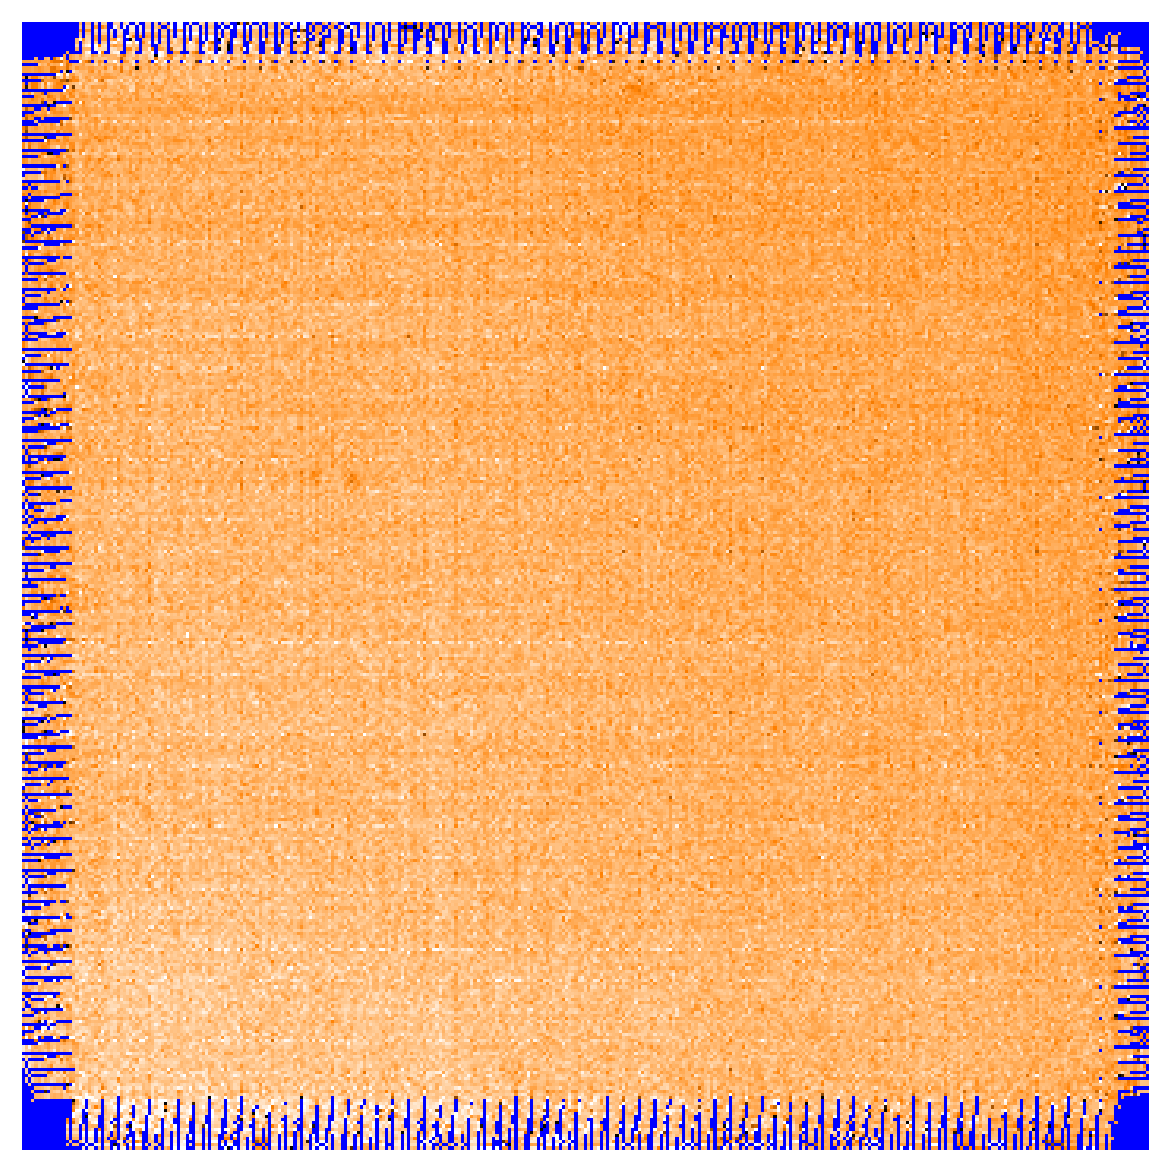
\includegraphics[width=5.2cm, height=5.2cm]{sc20_sincsinc.eps}
\label{fig:spread}
\caption[Options for the \makecube\ parameter `spread']{Raster map regridded with \makecube\ and \param{spread = nearest} (left), \param{Gauss} (centre) and \param{SincSinc} (right). Blank pixels are coloured blue. You can see the Nearest option has resulted in multiple blank pixels throughout the map.}
\end{center}
\end{figure}



\subsubsection{Generating a variance map}
The option  \param{genvar} can be used to generate a variance array for your cube. This is important if you are adding multiple maps with different variances as it allows them to be accurately weighted. There are three options for  \param{genvar}:

\begin{center}
\begin{minipage}[t]{0.12\linewidth}
\textbf{Spread}
\end{minipage}
\begin{minipage}[t]{0.8\linewidth}
The output variance values are based on the spread of input data values contributing to each output pixel. Note that this option is not available if parameter  \param{sparse} is set \param{true}. If the  \param{badmask} value is \param{or} or \param{first}, then a single variance value will be produced for each output spectrum. However, when \param{badmask} is \param{and} an independent variance value is calculated for each channel in each output spectrum.
\end{minipage}
\vspace{0.7cm}\\
\begin{minipage}[t]{0.12\linewidth}
\textbf{Tsys}
\end{minipage}
\begin{minipage}[t]{0.8\linewidth}
The output variance values are based on the system noise temperature values supplied in the input NDFs. Since each input spectrum is characterised by a single Tsys value, each output spectrum will have a constant Variance value (i.e. all channels in an output spectrum will have the same variance value). [Default]. 
\end{minipage}
\vspace{0.7cm}\\
\begin{minipage}[t]{0.12\linewidth}
\textbf{None}
\end{minipage}
\begin{minipage}[t]{0.8\linewidth}
 No output variance values are created.\\
\end{minipage}
\end{center}

\subsubsection{Sparse grid}
If one has observed a number of offset positions which are not on a regular grid or are widely spaced, it is of little use to make a normal cube with \makecube, which then would have a large size and which would be mostly empty. Then one can use the \makecube\ parameter  \param{sparse}. When \param{sparse=true} a one-dimensional array is created which stacks spectra in the order in which they were observed (from left to right when viewed with \gaia). 
{\color{MidnightBlue}\begin{myquote}
\begin{verbatim}
% smurfhelp makecube param sparse 
\end{verbatim}
\end{myquote}}
This is generates a one-dimensional array where spectra are displayed by \gaia\ in the order where they were observed (from left to right).

\subsubsection{Creating a catalogue of receptor positions}
You can use the option \param{outcat} to generate a catalogue of the spatial potions of the receptors used to make your final cube. The label associated with each row in the catalogue is the detector name. The detector positions in the catalogue are ordered as follows: all the positions for the first input NDF come first, followed by those for the second input NDF, etc. Within the group of positions associated with a single input NDF, the positions for the first time slice come first, followed by the positions for the second time slice, etc. 

{\color{MidnightBlue}\begin{myquote}
\begin{verbatim}
% makecube in=rawfiles outcat=cat
\end{verbatim}
\end{myquote}}

The catalogue produced will be in FITS format. In the example above a file called cat.FIT is created. When viewing your map with \gaia\ this catalogue can be overlaid to identify the receptors contributing to each pixel (see Figure \ref{fig:makecube-outcat}). 

\myfig{sc20_makecube-outcat}{[h!]}{width=1\linewidth}{fig:makecube-outcat}{Displaying receptor positions in \gaia.}{
 The receptor positions overlaid on a regridded cube of a HARP stare observation. This is viewed in \gaia\ by selecting Data-Servers $>$ Local Catalogs and selecting your \param{outcat} filename (here \param{cat.FITS}). Notice that dead receptors are excluded from the list.}

\subsubsection{Tile dimensions}
You can set the maximum tile size in pixels with the  \param{tiledims} option. This allows you to break a large raster map into smaller tiles with which can be abutted later.  Each tile comes with a rim of extra data to allow for future coadding.



\clearpage
\section{\xlabel{analyse}Analysing your Cube}
\label{sec:analyse}

\subsection{Smoothing your data}
Frequency or velocity smoothing is performed using \Kappa:\block. It uses a rectangular box filter with each output pixel either the mean or the median of the input pixels within the filter box. The box size can be set to 1 for dimensions which do not require smoothing. In the example below the spatial pixels remain untouched while the velocity axis is smoothed using a box of 5 channels.
{\color{MidnightBlue}\begin{myquote}
\begin{verbatim}
% block in=mycube out=rebinnedcube box="[1,1,5]"
\end{verbatim}
\end{myquote}}

Two-dimensional NDFs can also be smoothed using \gausmooth. This smooths using a symmetrical Gaussian point spread function (PSF) of specified width(s) and orientation. Each output pixel is the PSF-weighted mean of the input pixels within the filter box. 

{\color{MidnightBlue}\begin{myquote}
\begin{verbatim}
% gausmooth in=mymap out=smoothedmap fwhm=3
\end{verbatim}
\end{myquote}}
Note that the \param{fwhm} option is given in the number of pixels. For example, to smooth a map with 4$''$ pixels by a 12$''$ Gaussian you would set \param{fwhm=3}.

\subsection{Removing a baseline}
Baselines should be removed using \Kappa:\mfittrend. This routine can fit polynomials up to order 15,  or cubic splines, to each spectrum in your cube. You can specify the ranges to fit via the \param{ranges} parameter, or you can allow them to be determined automatically (\param{auto}). 

{\color{MidnightBlue}\begin{myquote}
\begin{verbatim}
% mfittrend in=cube ranges=\"-50 -10 80 160\" order=1 axis=3 out=baselinedcube
\end{verbatim}
\end{myquote}}

If using automatic range determination you should set the \param{numbin} option. This is the number of bins in which to compress the trend line. A single line or average may be noisy so binning is used to improve the signal-to-noise in order to enhance features which should be masked. 

Ideally the bin size should match your line width to get maximum single to noise between the emission and the background. Be aware that bins that are too big can dilute weaker features. Likewise, bins that are too small will get noisy at the edges of broad lines. We recommend you experiment with the bin size to find the best fit for your data.

To exclude features that are not part of the baseline trend you can use the \param{clip} option. Use \param{clip} to provide an array of standard deviations for progressive clipping of outliers within each bin. Once the data have been binned a trend is fit within each bin and the outliers clipped, the trend is then re-fitted and the outliers again clipped etc. By default this will clip at 2, 2, 2.5 and 3\,$\sigma$ successively but you may wish to experiment with your own clip levels. The \param{clip} option is only used when \param{auto=true}.
\\*\\*
\textbf{Advanced method}\\*
These steps give a more in depth way of determining the baselines and mimic the the pipeline.

\begin{enumerate}[label=(\arabic*)]
\item Perform a \block\ smooth on your reduced cube. Here the smoothing is quite aggressive with a box filter of 5  pixels along the spatial axes and 15 pixels along the frequency axis. This is to really pull out all emission features. You can tweak these to suit your data, e.g a narrower box might be needed if you have very narrow lines.
{\color{MidnightBlue}\begin{myquote}
\begin{verbatim}
% block in=cube out=temp1 box="[5,5,15]" estimator=mean
\end{verbatim}
\end{myquote}}

\item Perform \mfittrend\ on your smoothed cube with a high-order polynomial and automatic range determination.
{\color{MidnightBlue}\begin{myquote}
\begin{verbatim}
% mfittrend in=temp1 out=temp2 axis=3 order=3 auto method=single \
  variance subtract=false mask=blmask
\end{verbatim}
\end{myquote}}

\item Add the baseline mask to your original unsmoothed cube.
{\color{MidnightBlue}\begin{myquote}
\begin{verbatim}
% add in1=cube in2=blmask out=temp3
\end{verbatim}
\end{myquote}}

\item Perform \mfittrend\ on your masked unsmoothed cube with a lower-order polynomial. This time fit the full range by setting \param{auto=false}.
{\color{MidnightBlue}\begin{myquote}
\begin{verbatim}
% mfittrend in=temp3 out=temp4 axis=3 order=1 auto=false ranges=\! \
  method=single variance=true subtract=false
\end{verbatim}
\end{myquote}}

\item Subtract the baseline from the original unsmoothed cube.
{\color{MidnightBlue}\begin{myquote}
\begin{verbatim}
% sub in1=cube in2=temp4 out=baselinedcube
\end{verbatim}
\end{myquote}}
\end{enumerate}

\textbf{What about findback?}\\*
The \cupid\ routine \findback\ offers an alternative for background subtraction however there are more limitations. It applies spatial filtering to remove structure with a size scale less than a specified box size. Within each box the values are replaced by the minimum of the input values. The data are then filtered again and this time replaced with the maximum in each box. 

Using \findback\ results in a baseline trend that hugs the lower limit of the noise and can contain sharp edges. These problems can be mitigated but extra steps are required. See \cupidsun\ for more details.

\subsection{Collapsing your map}

An integrated intensity map can be created by collapsing your cube along the frequency/velocity axis using  \Kappa:\collapse. For each output pixel, all input pixels between the specified bounds are collapsed and combined using one of a selection of estimators. Amongst others, the estimators include the mean, integrated value, maximum value, the mean weighted by the variance, RMS value and total value. See \kappasun\ for a full list.

The example below includes the options \param{low} and \param{high} which can be specified to limit the range over which the cube is collapsed on the given axis (in this case from -5\,km/s to +10\,km/s). The \param{variance} flag indicates the variance array should be used to define weights and generate an output variance. The option \param{wlim} sets the fraction of pixels that must be `good' in the collapse range for a valid output pixel to be generated. You may find you need to reduce the value for \param{wlim} below its default of 0.3 for some data.

{\color{MidnightBlue}\begin{myquote}
\begin{verbatim}
% collapse in=cube axis=vrad estimator=integ variance=true low=-5.0 high=10.0 \
  wlim=0.5 out=integmap
\end{verbatim}
\end{myquote}}
If you do not know the axis name you can give the number instead (1=RA, 2=Dec, 3=vrad).
\\*\\*
\textbf{Advanced method}\\*
These steps mimic the pipeline and show the procedure for generating an integrated map collapsed only over regions with emission greater than 3\,$\sigma$.

\begin{enumerate}[label=(\arabic*)]
\item Use \findclumps\ to run a clump-finding algorithm on your cube. Specify the 3\,$\sigma$ limit in your configuration file. See Section \ref{sec:clumpfind} for more details on clump-finding and Section \ref{sec:noise} for how to determine your RMS.
{\color{MidnightBlue}\begin{myquote}
\begin{verbatim}
% findclumps in=cube rms=<medianrms> config=^myconfig.dat \
  method=clumpfind out=temp1 outcat=mycat deconv=no
\end{verbatim}
\end{myquote}}

\item Divide the map by itself to create a clump mask that has clump regions set to 1.
{\color{MidnightBlue}\begin{myquote}
\begin{verbatim}
% div in1=temp1 in2=temp1 out=temp2
\end{verbatim}
\end{myquote}}

\item Set the bad data to zero using \Kappa:\nomagic.
{\color{MidnightBlue}\begin{myquote}
\begin{verbatim}
% nomagic in=temp2 out=temp3 repval=0
\end{verbatim}
\end{myquote}}

\item Multiply your reduced cube by the clump mask.
{\color{MidnightBlue}\begin{myquote}
\begin{verbatim}
% mult in1=cube in2=temp3 out=maskedcube
\end{verbatim}
\end{myquote}}

\item Collapse your masked reduced cube.
{\color{MidnightBlue}\begin{myquote}
\begin{verbatim}
% collapse in=maskedcube out=integ estimator=integ wlim=0.1 variance
\end{verbatim}
\end{myquote}}
\end{enumerate}

\subsubsection{Moments Maps}
You can use \collapse\ to generate the moments maps by selecting the appropriate \param{estimator} option --  Integrated value (Integ) for the integrated map (0th moment), Intensity-weighted co-ordinate (Iwc) to get the velocity field (1st moment), or Intensity-weighted dispersion (Iwd) to get the velocity dispersion (2nd moment).

\begin{latexonly}
\begin{center}
\begin{fmpage}{0.95\linewidth}
\vspace{0.1cm}
TIP: You can also use the \picard\ recipe CREATE\_MOMENTS\_MAPS. See \cref{Appendix}{app:picard}{Picard} for details. This recipe follows the advanced method outlined above.
\end{fmpage}
\end{center}
\end{latexonly}

\begin{htmlonly}
\textbf{TIP: You can also use the \picard\ recipe CREATE\_MOMENTS\_MAPS. See \cref{Appendix}{app:picard}{Picard} for details.  This recipe follows the advanced method outlined above.\\*\\*}
\end{htmlonly}


\subsection{\xlabel{rebin}Main beam conversion}
\label{sec:mult}
Your cube will come out of \makecube\, and the pipeline, in units of $T_A^*$. To convert this to main beam temperature, $T_{MB}$ multiply your cube by the main beam efficiency, $\eta_{MB}$. Alternatively, to convert to receiver temperature, $T_{rec}$, multiply by the forward scattering and spillover efficiency, $\eta_{fss}$.  See \cref{Section}{sec:instruments}{Heterodyne instruments} for efficiency values for RxA and HARP, and the JCMT webpages for further information and historical numbers.

You can use the \Kappa\ command \cmult\ to multiply any NDF by a constant.

{\color{MidnightBlue}\begin{myquote}
\begin{verbatim}
% cmult in=harpcube 0.63 out=harpcube_Tmb 
\end{verbatim}
\end{myquote}}

\subsection{\xlabel{rebin}Changing the pixel size}
\label{sec:rebin}
You may want to regrid your data onto larger pixels, for instance to allow direct comparison with data from other observatories. In the example below a JCMT map is regridded and aligned to match a Herschel map. See Appendix \ref{app:convert} for instructions on converting your FITS file to NDF format.
{\color{MidnightBlue}\begin{myquote}
\begin{verbatim}
% wcsalign in=jcmtmap out=regridmap lbnd=! ubnd=! ref=herschelmap rebin conserve=f
\end{verbatim}
\end{myquote}}

Alternatively, to resample your data onto smaller pixels you should use the \Kappa\ command \sqorst. In the example below 'map' has a pixel size of 8$''$, while `resamplemap' has a pixel size of 4$''$ -- the number of pixels has been doubled by applying a factor of 2 to the spatial axes. A factor of 1 was applied to the frequency (third) axis leaving it unchanged.
{\color{MidnightBlue}\begin{myquote}
\begin{verbatim}
% sqorst in=map out=resamplemap factors="[2,2,1]" conserve
\end{verbatim}
\end{myquote}}
\param{mode=factors} is the default setting so it was not specified in the example above. The example below however, uses  \param{mode=pixelscale} to  define a pixel size for the third axis; here the spectra are rebinned into 2\,km/s channels.
{\color{MidnightBlue}\begin{myquote}
\begin{verbatim}
% sqorst in=map out=resamplemap mode=pixelscale pixscale=2 axis=3
\end{verbatim}
\end{myquote}}

Remember you can check your current pixel size and channel spacing with \ndftrace\ (see \cref{Section}{sec:fitslist}{How can I view the metadata?}).

\subsection{\xlabel{mosaic}Mosaicking cubes}
\label{sec:mosaic} 
If you pass raw files covering different regions of the sky to \makecube\ it will automatically mosaic them together. This can be heavy work for your processor so you may wish to make individual cubes and combine them during post-processing. To coadd multiple reduced maps you should use \wcsmosaic. 
{\color{MidnightBlue}\begin{myquote}
\begin{verbatim}
% wcsmosaic in=^maplist out=mosaic lbnd=! ubnd=! variance
\end{verbatim}
\end{myquote}}
By selecting the lower bound (\param{lbnd}) and upper bound  (\param{ubnd}) to be default (!) you are including all of the input tiles. You can change these if you want to only mosaic a sub-region of the input maps. As with \makecube\ there are a number of regridding options available to you describing how to divide an input pixel between a group of neighbouring output ones (the default is \param{SincSinc}).


\begin{latexonly}
\begin{center}
\begin{fmpage}{0.95\linewidth}
\vspace{0.1cm}
TIP: Take care not to combine data separated on the sky as \wcsmosaic\ will attempt to create a vast cube that encompasses all the input files until it runs out of resources.
\end{fmpage}
\end{center}
\end{latexonly}

\begin{htmlonly}
\textbf{TIP: Take care not to combine data separated on the sky as \wcsmosaic\ will attempt to create a vast cube that encompasses all the input files until it runs out of resources.\\*\\*}
\end{htmlonly}


\begin{latexonly}
\begin{center}
\begin{fmpage}{0.95\linewidth}
\vspace{0.1cm}
TIP: You can also use the \picard\ recipe MOSAIC\_JCMT\_IMAGES. This will correctly combine all NDF extensions. See \cref{Appendix}{app:picard}{Picard} for details. 
\end{fmpage}
\end{center}
\end{latexonly}

\begin{htmlonly}
\textbf{TIP: You can also use the \picard\ recipe MOSAIC\_JCMT\_IMAGES. This will correctly combine all NDF extensions. See \cref{Appendix}{app:picard}{Picard} for details. \\*\\*}
\end{htmlonly}


\subsection{\xlabel{Crop}Cropping your map}
\label{sec:collapse}
Cropping an ACSIS map can be fiddly. The simplest way is to create an ARD mask in \gaia\ and apply it to your map. The steps below work on both two- and three-dimensional data.

\begin{enumerate}[label=(\arabic*)]
\item Create your ARD mask. You may find it easiest to do this with \gaia. See Figure \ref{fig:ardmask} for an illustrated guide.

\item Trim off the third axis from your mask using \ndfcopy.
{\color{MidnightBlue}\begin{myquote}
\begin{verbatim}
% ndfcopy mask trim trimwcs
\end{verbatim}
\end{myquote}}

\item Apply the saved ARD mask to your map. Setting \param{inside=false} will mask the pixels outside rather than inside your mask. The masked pixels will appear blank when you open it with \gaia; see the left-hand panel of Figure \ref{fig:crop}.
{\color{MidnightBlue}\begin{myquote}
\begin{verbatim}
% ardmask map inside=false ard=ardmask.txt out=maskmap
\end{verbatim}
\end{myquote}}

\item Trim off the blank pixels using \ndfcopy\ with the \param{trimbad} option. This leaves just your selected region; see the right-hand panel of Figure \ref{fig:crop}.
{\color{MidnightBlue}\begin{myquote}
\begin{verbatim}
% ndfcopy maskmap trimbad
\end{verbatim}
\end{myquote}}
\end{enumerate}

An alternative method is to use \ndfcopy\ while defining the section of the map or cube you wish to extract as an output cube. See \cref{Section}{sec:ndfsections}{How to examine, process or extract a subset of your data}.
\vspace{3mm}\\
\textbf{Supplying a template}\\*
If you wish to extract only a region which overlaps with an existing file you have, e.g. from a different observing campaign or telescope, you can also use \ndfcopy\ but with the \param{like} option.
{\color{MidnightBlue}\begin{myquote}
\begin{verbatim}
% ndfcopy in_full out_cropped like=map2 likewcs
\end{verbatim}
\end{myquote}}
The shape of the file supplied by  \param{like} will determine the shape of the output file. This shape can be in either pixel indices or the current WCS Frame. If the WCS Frame is required, include the parameter \param{likewcs} to the command line otherwise it can be omitted.


\begin{latexonly}
\begin{figure}[ht!]
\begin{center}
\begin{fmpage}{0.99\linewidth}
\vspace{0.2cm}
\hspace{0.2cm}
\textbf{Defining an ARD region in \gaia}

\vspace{0.5cm}
\hspace{0.1cm}
\begin{minipage}[c]{0.23\linewidth}
Open your map with \gaia.
\end{minipage}
\hspace{0.2cm}
\begin{minipage}[c]{0.72\linewidth}
{\color{MidnightBlue}\begin{myquote}
\begin{verbatim}
% gaia map
\end{verbatim}
\end{myquote}}
\end{minipage}

\vspace{0.5cm}
\hspace{0.1cm}
\begin{minipage}[c]{0.23\linewidth}
In \gaia\ go to \gaiathing{Image-analysis$>$Image regions}.
\end{minipage}
\hspace{0.2cm}
\begin{minipage}[c]{0.72\linewidth}
\centering
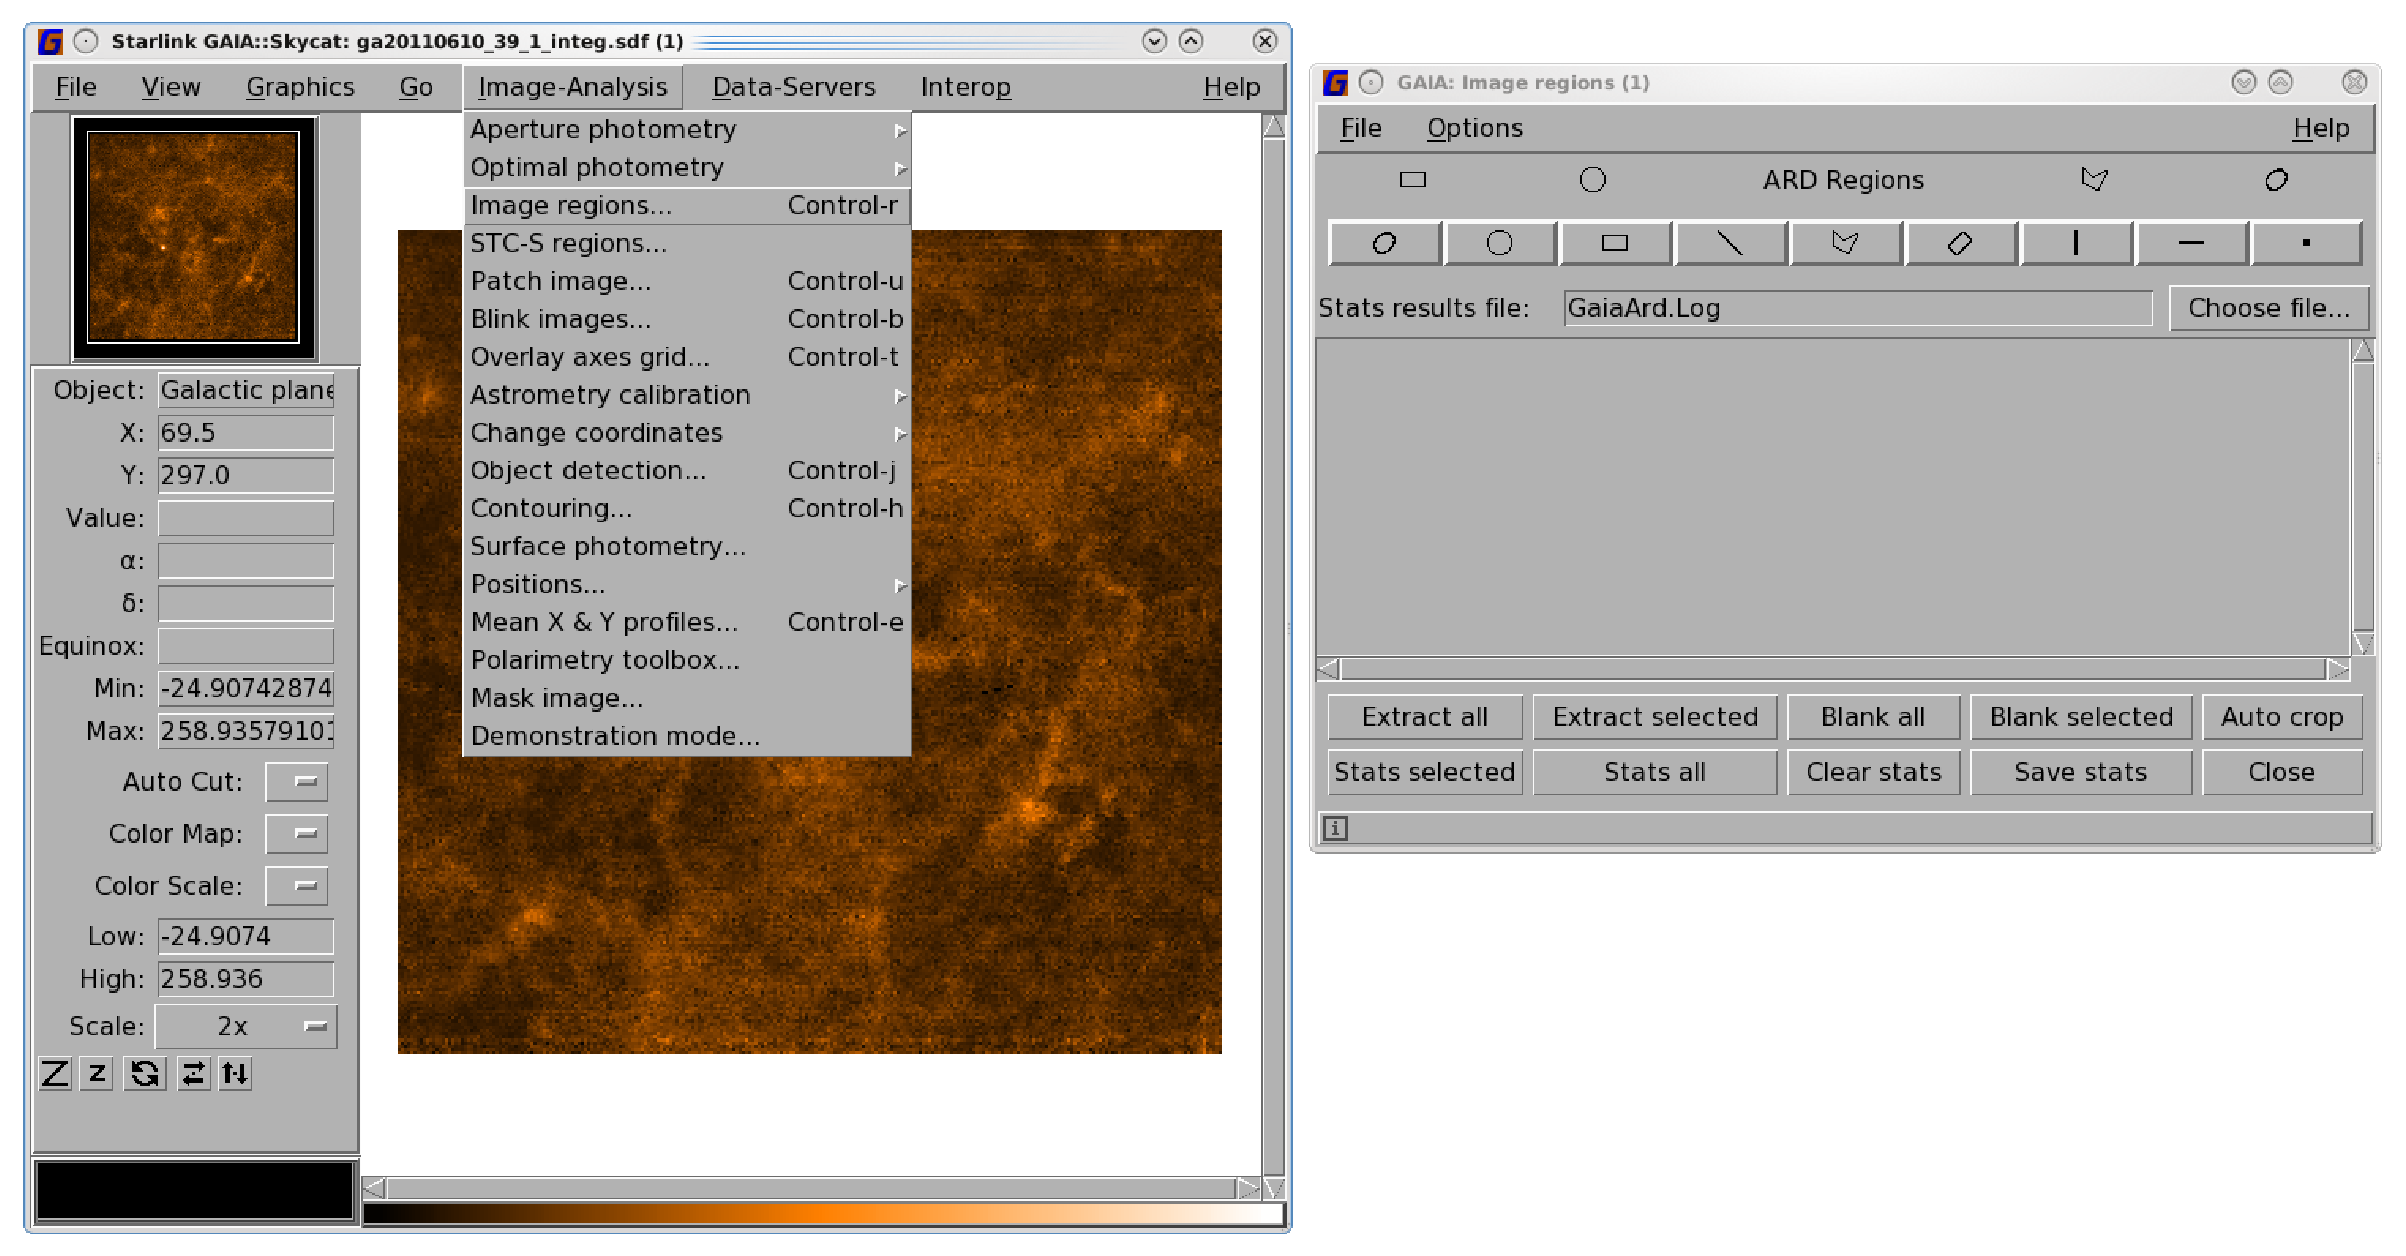
\includegraphics[width=0.98\textwidth]{sc20_ard7.eps}
\end{minipage}

\vspace{0.5cm}

\hspace{0.1cm}
\begin{minipage}[c]{0.23\linewidth}
Select the shape of the ARD region you wish to define and drag it on your map by holding the mouse button down, dragging the shape out, then releasing the button. 
\end{minipage}
\hspace{0.2cm}
\begin{minipage}[c]{0.72\linewidth}
\centering
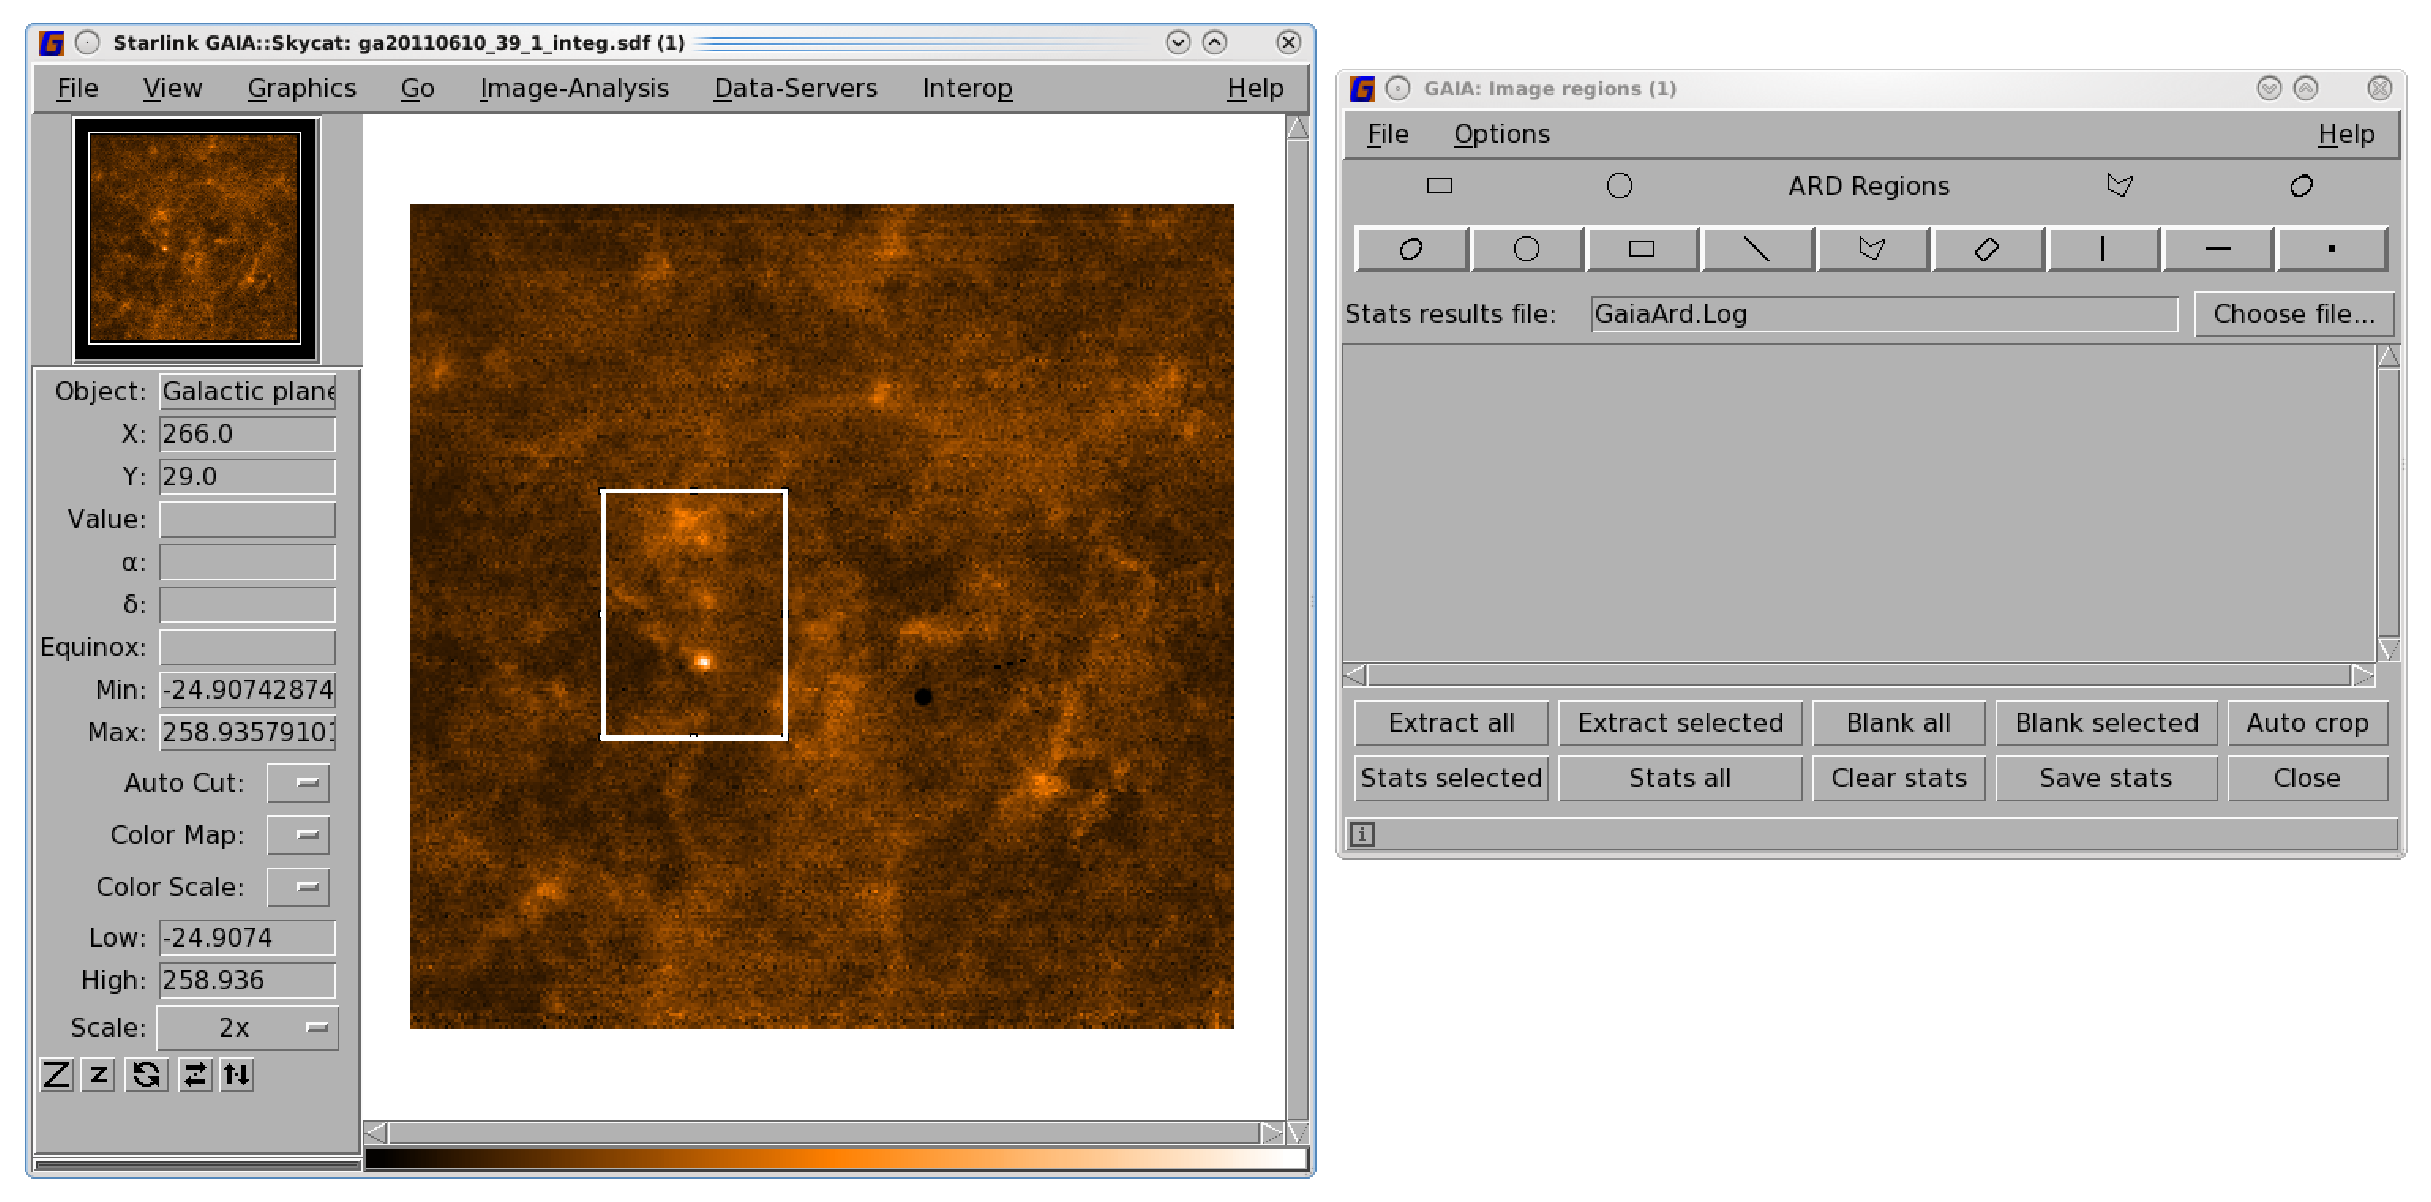
\includegraphics[width=0.98\textwidth]{sc20_ard3.eps}
\vspace{0.2cm}
\end{minipage}

\vspace{0.5cm}


\hspace{0.1cm}
\begin{minipage}[c]{0.23\linewidth}
In the \gaiathing{Image regions} window go to \gaiathing{File$>$Save ARD description} to save your ARD mask for later use.
\end{minipage}
\hspace{0.2cm}
\begin{minipage}[c]{0.72\linewidth}
\centering
\includegraphics[width=0.98\textwidth]{sc20_ard4.eps}
\vspace{0.2cm}
\end{minipage}

\end{fmpage}
\end{center}
\caption[Defining an ARD region using \gaia]{\small Defining an ARD region using \gaia.}
\label{fig:ardmask}
\end{figure}
\end{latexonly}


\begin{figure}[h!]
\begin{center}
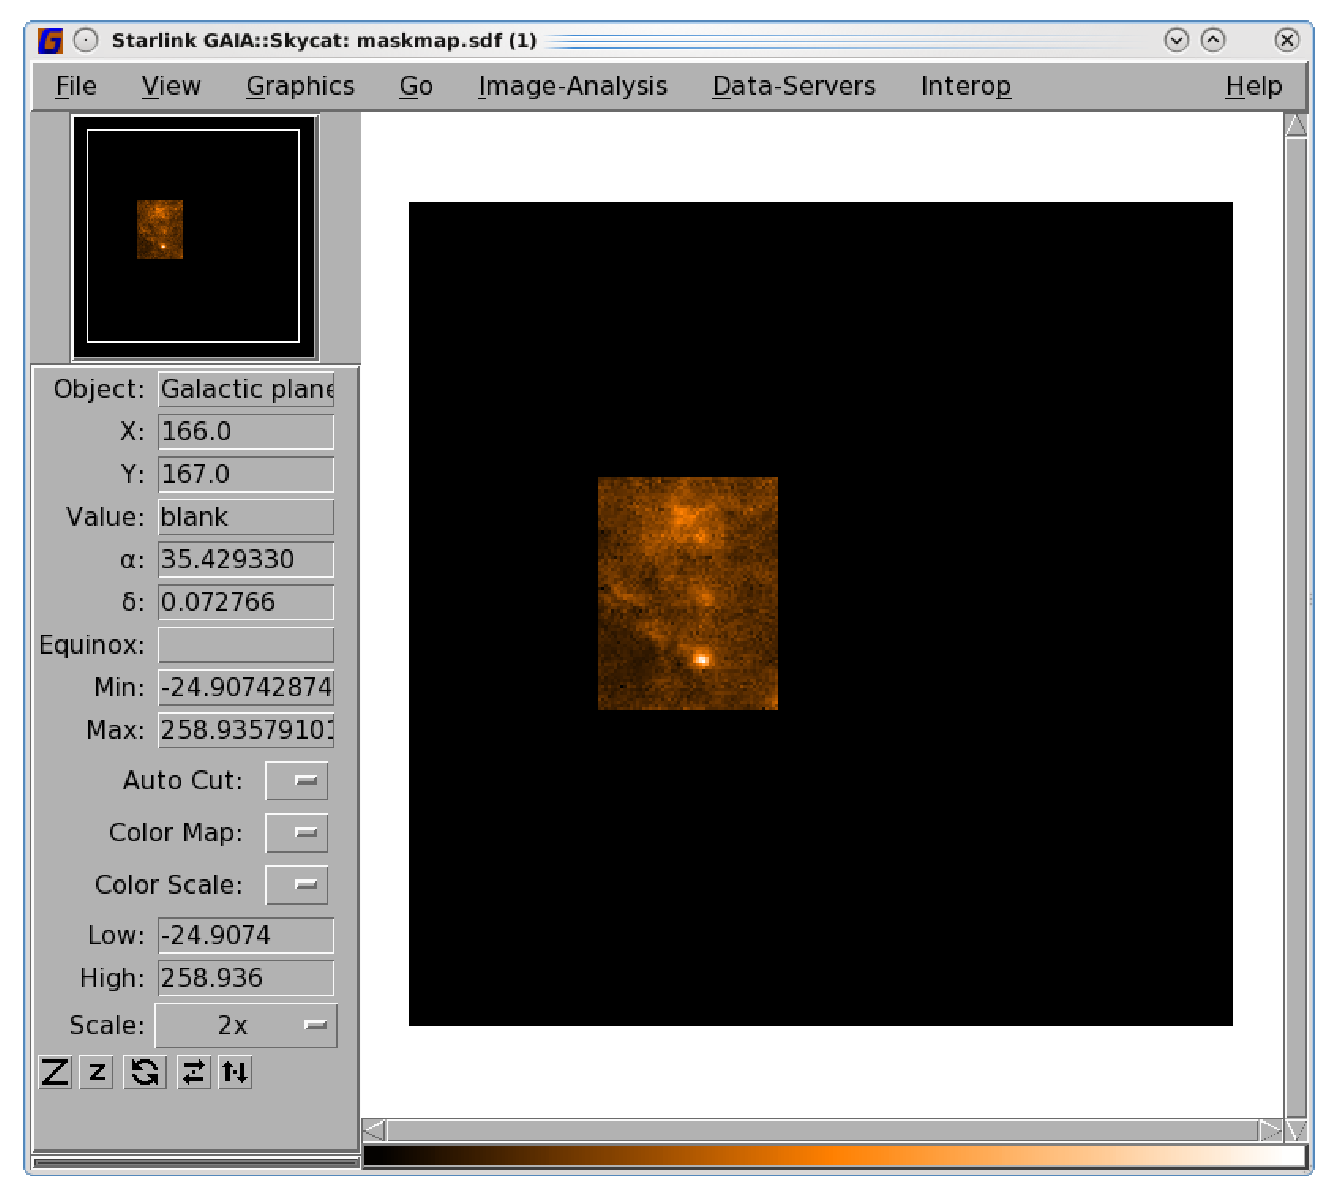
\includegraphics[height=7cm]{sc20_ard5.eps}
\hspace{0.3cm}
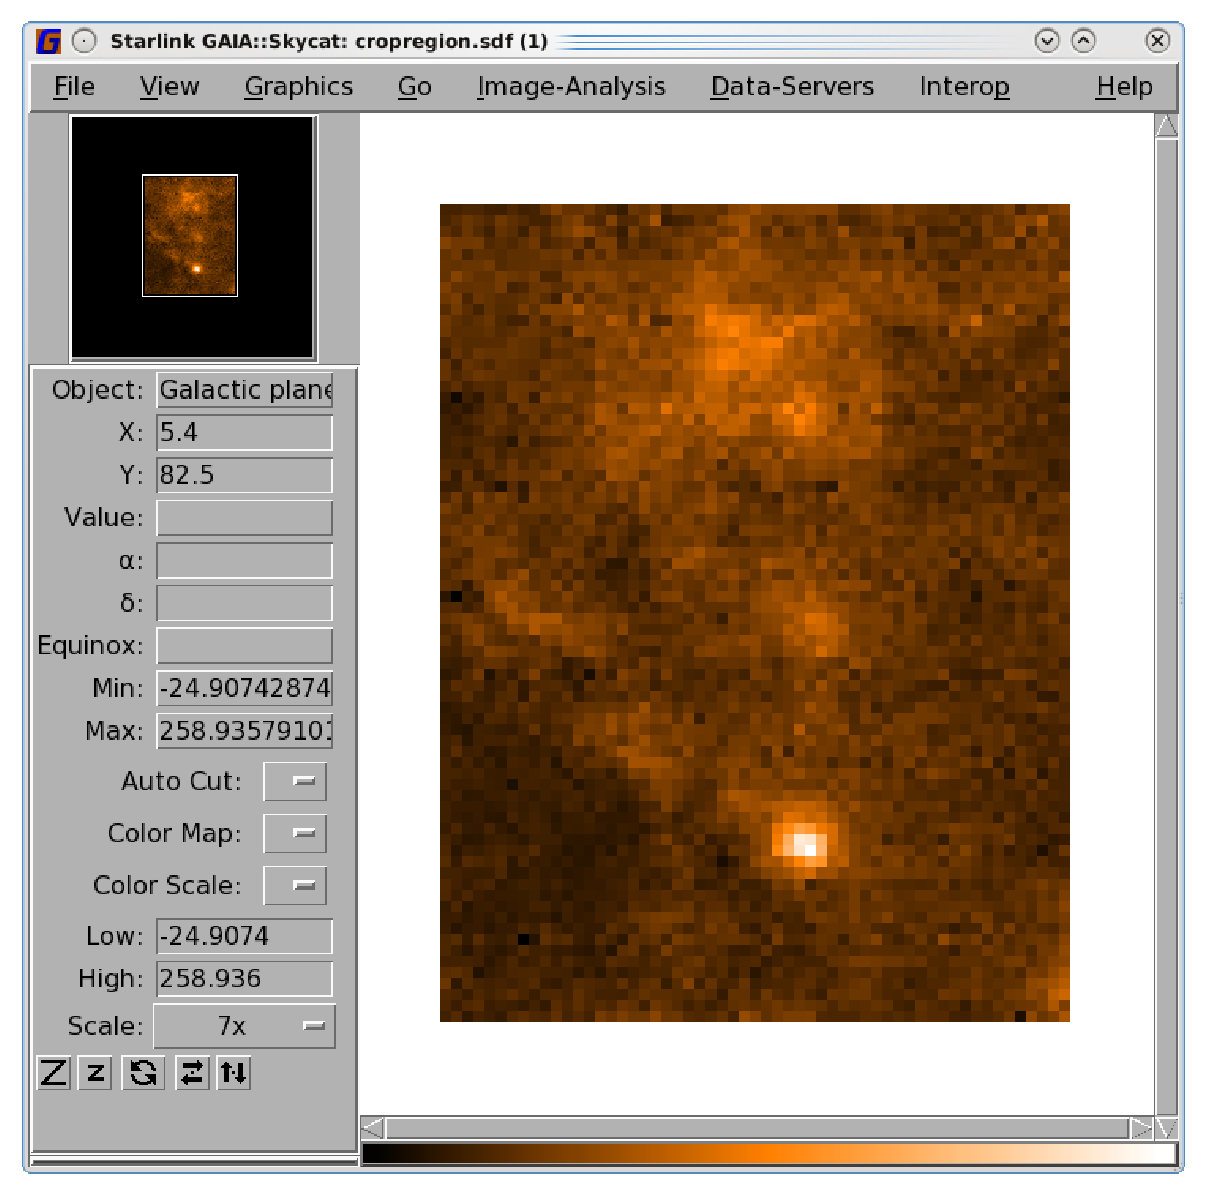
\includegraphics[height=7cm]{sc20_ard6.eps}
\caption[Cropping a region of a 2D map.]{(Left) After applying the ARD mask, the cropped region is still surrounded by blank pixels. (Right) The blank pixels have been trimmed using \ndfcopy\ with the \param{trimbad} option.}
\label{fig:crop}
\end{center}
\end{figure}


\subsection{\xlabel{holes}Filling holes in your map}
\label{sec:holes}

You may come across empty pixels in your map due to dead receptors or receptors which have failed quality assurance in the pipeline. The second half of 2013 in particular had only 12 working receptors for HARP.   

You can fill these holes using \Kappa:\fillbad. This replaces the bad values with a smooth function derived from neighbouring values, derived by iterating to a solution of Laplace's equation.

The default values for \fillbad\ will fill the holes but smooths by 5 pixels along each axis. If you prefer not to smooth in the spectral axis, set the parameter \param{size} to [s,s,0] where s is the scale length in pixels.  The zero means do not smooth along the third axis. 

The scale length should have a value about half the size of the largest region of bad data to be replaced.  Since the largest bad regions apart from the cube peripheries are two pixels across, a size of 1 is appropriate.
{\color{MidnightBlue}\begin{myquote}
\begin{verbatim}
% fillbad in=holeymap out=filledmap  size="[1,1,0]"
\end{verbatim}
\end{myquote}}
\cref{Figure}{fig:fillholes}{The figure below} shows an initial map with holes and the final filled map.

\myfigduo{sc20_holeyharp}{sc20_polyfillaharp}{[h!]}{width=0.48\linewidth}{fig:fillholes}{0.5mm}{Filling holes in your HARP map with \fillbad.}{Filling holes in your HARP map with \fillbad. Compare the original map (left) to the filled map (right).}


\subsection{\xlabel{noise}Checking the noise}
\label{sec:noise}
You can use  \Kappa:\stats\ to check the noise in your map. It will report the statistics for all pixels so be aware that noisy edges and strong signal will contribute to the standard deviation. You can mitigate this by trimming any noisy edges and by examining the square root of the Variance component (hereafter referred to as the error component\footnote{No such component exists in the NDF.}) although bright emission will still increase your noise. You can select the error component with \param{comp=err} on the command line.
{\color{MidnightBlue}\begin{myquote}
\begin{verbatim}
% stats file comp=err order
\end{verbatim}
\end{myquote}}
Including the option \param{order} allows the ordered statistics such as the median and percentiles to be reported. Note that percentile options will need to be specified via the \param{percentiles} parameter.
\begin{latexonly}
\begin{center}
\begin{fmpage}{0.95\linewidth}
\vspace{0.1cm}
TIP: Remember the mean or median values will give you the noise when using the error component.
\end{fmpage}
\end{center}
\end{latexonly}

\begin{htmlonly}
\textbf{TIP: Remember the mean or median values will give you the noise when using the error component.\\*\\*}
\end{htmlonly}

\vspace{3mm}
\textbf{Visualising the noise}\\
You can plot the noise or error component of your map using the
\textsc{Kappa} command \histogram. This allows you to visualise the
distribution with more ease. Again the \param{comp=err} option is
used.
{\color{MidnightBlue}\begin{myquote}
\begin{verbatim}
% histogram mosaic comp=err range=! numbin=200 
\end{verbatim}
\end{myquote}}
The output is shown in \cref{Figure}{fig:noihisto}{the graphic below}. An alternative to setting the number of bins via the \param{numbin} parameter is to set the width of each bin using the \param{width} parameter.

\myfig{sc20_noihisto1}{[h!]}{width=0.6\linewidth}{fig:noihisto}{A histogram of the error component.}{The error component plotted with \histogram.}

It is also useful to view the noise map itself. \cref{Figure}{fig:noisemap}{The figure below} shows how to select the error component in \gaia. Other options available from the \gaiathing{Select NDF in container file} window include the exposure time, the effective time and, if \param{spread=nearest} when running \makecube, the system temperature. To return to your main image select the top level and click the \gaiathing{Data} button.

\begin{latexonly}
\begin{center}
\begin{fmpage}{0.95\linewidth}
\vspace{0.1cm}
TIP: You can write out the error component into a new file using \ndfcopy. \texttt{\% ndfcopy map comp=err noisemap}
\end{fmpage}
\end{center}
\end{latexonly}

\begin{htmlonly}
\textbf{TIP: You can write out the error component into a new file using \ndfcopy. \texttt{\% ndfcopy map comp=err noisemap}}
\end{htmlonly}


\myfig{sc20_noimap}{[h!]}{width=0.6\linewidth}{fig:noisemap}{The noise map of a mosaic of tiles.}{The noise map of a mosaic of tiles taken in differing weather conditions.}


\clearpage
\section{\xlabel{advanced}Advanced Analysis}
\label{sec:advanced}

\subsection{\xlabel{coords}Changing coordinate frames}
Coordinate systems of regridded Starlink files are described by the world coordinate system, (WCS). There are a number of basic coordinate systems (or frames) common to all NDFs; these are described by their DOMAIN (essentially their name) and are PIXEL, AXIS, GRID and FRACTION. Additional frames can be stored in the WCS  component. Two common additional frames are SKY and SPECTRUM. SKY refers to two-dimensional frames (known as SkyFrames) which describe sky coordinates. SPECTRUM refers to one-dimensional frames (known as SpecFrames) that describe a position within a spectrum.

The choice of coordinates within the SkyFrame or SpecFrame is called the system. For example, for SkyFrames this may be Galactic or FK5, while for SpecFrames this may be velocity or frequency.

The current frame and the system can both be changed using the  \Kappa\ applications \wcsframe\ and \wcsattrib. The current frame for data processed with \makecube\ (either manually or by the pipeline) typically has a DOMAIN of SKY-DSBSPECTRUM. The compound name refers to the first two axes of the frame having sky coordinates and the third axis having dual side-band spectral units. You can check this with \ndftrace:

{\color{MidnightBlue}\begin{myquote}
\begin{verbatim}
% ndftrace file.sdf | grep Domain
\end{verbatim}
\end{myquote}}
You can change the attributes of a cube using \wcsattrib. To change the SkyFrame coordinate system set the \param{system} attribute.
{\color{MidnightBlue}\begin{myquote}
\begin{verbatim}
% wcsattrib file.sdf set system galactic
\end{verbatim}
\end{myquote}}
To change between velocity and frequency you also use the  \param{system} attribute. For SKY-DSBSPECTRUM the software knows which axis is being referred to based on the option you supply (the third in this case).
{\color{MidnightBlue}\begin{myquote}
\begin{verbatim}
% wcsattrib file.sdf set system freq
% wcsattrib file.sdf set system vrad
\end{verbatim}
\end{myquote}}
Once a cube has been collapsed and is two-dimensional its frame becomes SKY. If you need to change frames manually use \wcsframe.
{\color{MidnightBlue}\begin{myquote}
\begin{verbatim}
% wcsframe file sky
\end{verbatim}
\end{myquote}}

For offset coordinates you will need to set the system \param{skyrefis} to origin. The final two lines in the example below convert the offset units to arcseconds instead of radians.
{\color{MidnightBlue}\begin{myquote}
\begin{verbatim}
% wcsattrib file.sdf set skyrefis origin
% wcsattrib file set 'format(1)' 's.*'
% wcsattrib file set 'format(2)' 's.*'
\end{verbatim}
\end{myquote}}

%
%\subsection{\xlabel{despike}Despiking}
%Interference spikes are sometimes found in ACSIS data. Spikes should be quite conspicuous in the data cube as they occur at the same frequency throughout the observed cube and at (almost) uniform intensity. It is probably best to eliminate spikes in your data cube from the raw time-series, i.e. before running \makecube\ or any other processing on your data. 
%
%If you suspect you have a spike in your data Appendix \ref{app:spike} describes the procedure for identifying the position of the spike and masking it out.
%

\subsection{\xlabel{hybrid}Hybrid Data}
To merge two hybrid observations first do \wcsalign\ on both files.
{\color{MidnightBlue}\begin{myquote}
\begin{verbatim}
% wcsalign in="'rawfile_01.sdf,rawfile_02.sdf'" insitu lbnd=! ubnd=! ref=!
\end{verbatim}
\end{myquote}}
Next trim each sub-system to remove noisy ends of the spectra in the overlap region. You can get the pixel bounds from \ndftrace\ (here 1024). The example below trims 35 channels from the `left' of rawfile\_01 and 24 channels from the `right' of rawfile\_02.
{\color{MidnightBlue}\begin{myquote}
\begin{verbatim}
% ndfcopy in='rawfile1_01(35:1024,,)'
% ndfcopy in='rawfile_02(0:1000,,)'
\end{verbatim}
\end{myquote}}
These can then be merged using \wcsmosaic.
{\color{MidnightBlue}\begin{myquote}
\begin{verbatim}
% wcsmosaic in='"rawfile1,rawfile2"' out=rawfile12 lbnd=! method=nearest accept
\end{verbatim}
\end{myquote}}
 You should check the final spectra to make sure there is no noise bump in the middle where they overlap.

\subsection{\xlabel{pv}Position-velocity diagram}
You can create a position-velocity map by collapsing over the skylat axis of a reduced cube. Use the \Kappa\ command \collapse\ with \param{axis=skylat}:

{\color{MidnightBlue}\begin{myquote}
\begin{verbatim}
collapse in=reduced.sdf axis=skylat estimator=sum out=pv
\end{verbatim}
\end{myquote}}
You can view your pv map with  \gaia\ or \display.

\subsection{\xlabel{channel}Creating channel maps}
\label{sec:channel}

The \Kappa\ application \chanmap\ creates a two-dimensional channel map from a cube. It collapses along the nominated axis (with many of the same parameters as \collapse). The number of channels to create is given by \textit{nchan} and these are divided evenly between your ranges. The arrangement of the resulting panels is determined by the shape parameter. The collapsed slices are tiled with no margins to form the final image.

{\color{MidnightBlue}\begin{myquote}
\begin{verbatim}
% chanmap in=cube axis=3 low=-10 high=5 nchan=6 shape=3 estimator=mean
\end{verbatim}
\end{myquote}}
This grid of channel maps is filled from left to right, and bottom to top. It can be viewed with \gaia\ (see Figure \ref{fig:chanmap}) or with \display.
{\color{MidnightBlue}\begin{myquote}
\begin{verbatim}
% display chanmap mode=faint noaxes lut=/star/bin/kappa/smooth3_lut.sdf
\end{verbatim}
\end{myquote}}

Channel maps can also be created using \gaia. See \cref{Section}{sec:gaiachannel}{Channel maps} for instructions.


\myfig{sc20_chanmap}{[h!]}{width=0.8\linewidth}{fig:chanmap}{Displaying a channel map with \gaia.}{Displaying a channel map with \gaia.}

\subsection{\xlabel{clumpfinding}Clump finding}
\label{sec:clumpfind}
The \cupid\ application \findclumps\ can be used to generate a clump catalogue. It identifies clumps of emission in one-, two- or three-dimensional NDFs. You can select from the clump-finding algorithms FellWalker, Gaussclumps, ClumpFind or Reinhold . You must supply a configuration file which lists the options for which ever algorithm you chose (see  the \xref{\textsc{cupid} manual}{sun255}{} for a full list). The result is returned as a catalogue in a text file and as a NDF pixel mask showing the clump boundaries (see Figure \ref{fig:clumps2}). See Appendix \ref{app:clumpfind} for descriptions of the various algorithms.

{\color{MidnightBlue}\begin{myquote}
\begin{verbatim}
% findclumps in=map.sdf out=clumpmap.sdf outcat=clumps.FIT logfile=clumps.log \
  config=^myconfig.dat method=clumpfind rms=0.2 shape=polygon
\end{verbatim}
\end{myquote}}

 The shape option allows \findclumps\ to create and STC-S description (polygonal or elliptical) for each clump found. These are added as extra columns to the output catalogue. 
\vspace{0.7cm}\\
\begin{minipage}[t]{0.12\linewidth}
\textbf{Polygon}
\end{minipage}
\begin{minipage}[t]{0.85\linewidth}
Each polygon will have, at most, 15 vertices. For two-dimensional data the polygon is a fit to the clump's outer boundary (the region containing all good data values). For three-dimensional data the spatial footprint of each clump is determined by rejecting the least significant 10\% of spatial pixels, where ``significance'' is measured by the number of spectral channels that contribute to the spatial pixel. The polygon is then a fit to the outer boundary of the remaining spatial pixels. 
\end{minipage}
\vspace{0.7cm}\\
\begin{minipage}[t]{0.12\linewidth}
\textbf{Ellipse}
\end{minipage}
\begin{minipage}[t]{0.85\linewidth}
All data values in the clump are projected onto the spatial plane and ``size'' of the collapsed clump at four different position angles -- all separated by 45$^\circ$ -- is found. The ellipse that generates the same sizes at the four position angles is then found and used as the clump shape. 
\end{minipage}
\vspace{0.7cm}\\
You can plot the clump outlines over an image using \gaia. See Section \ref{sec:plotclumps} for instructions.

\vspace{0.7cm}
\myfig{sc20_clumps}{[h!]}{width=0.7\linewidth}{fig:clumps2}{A velocity slice of the result of 3D clump finding viewed with \gaia.}{A velocity slice of the result of 3D clump finding viewed with \gaia. This output NDF contains boundaries of the clumps with the value reflecting the number of pixels contained within that clump.}


\clearpage
\section{\xlabel{gaia}Using GAIA}
\label{sec:gaia}

\subsection{Removing a baseline with GAIA}
\begin{enumerate}[label=(\textbf{\arabic*})]
\item Select the spectrum you want to use as your template for the entire cube.

\item Select the Baseline tab in the \gaiathing{Display image regions} window.

\item Select the order of the baseline you want to fit and remove

\item Check the \gaiathing{Show limits on plot} button to interactively draw your baseline windows. You can click and drag the edges of these limit lines in the \gaiathing{Spectral plot} window.

\item Check \gaiathing{Enable} for each new baseline window you want to define.

\item Click \gaiathing{Run}.
\end{enumerate}

\myfig{sc20_gaia_baseline}{[h!]}{width=0.9\linewidth}{fig:gaiabaseline}{Removing a baseline with \gaia.}{Removing a baseline with \gaia.}

\subsection{Creating channel maps with GAIA}
\label{sec:gaiachannel}
You can display channel maps in \gaia\ by selecting the region of a spectrum you wish to collapse over. You can use a spectrum from any of the pixels in the cube and the region selected will be applied to the whole map.

\begin{enumerate}[label=(\textbf{\arabic*})]
\item  Select the spectrum you want to use as your template for the entire cube.

\item Select the \gaiathing{Chanmap} tab in the \gaiathing{Display image regions} window.

\item Check the \gaiathing{Show limits on plot} box to interactively draw the range over which to collapse your cube. You can click and drag the end-bars of the limit lines in the \gaiathing{Spectral plot} window.

\item Select the collapse method (Max is chosen in the example).

\myfig{sc20_gaia_channel1}{[h!]}{width=0.93\linewidth}{fig:gaia_chan1}{Creating a channel map with \gaia.}{Creating a channel map with \gaia.}

\item Use the slider bars to select the total number of channels you want to generate and the number of \texttt{x}-axis channels. The \texttt{x}-axis channel number sets the aspect ratio for the resulting display grid.

\item Click \gaiathing{Run}. The result is shown in the figure below.

\myfig{sc20_gaia_channel2}{[t!]}{width=0.6\linewidth}{fig:gaia_chan2}{Channel map created with \gaia.}{Channel map created with \gaia.}
\end{enumerate}


\subsection{Contouring with GAIA}
\begin{enumerate}[label=(\textbf{\arabic*})]
\item  Open the map you wish to contour over.

\item Select \gaiathing{Image-Analysis$>$Contouring} from the menu bar across the top of the main window.

\item Select the file you wish to contour in the \gaiathing{Contouring} window.

\item Generate your contours in the \gaiathing{Generate} tab found on the left-hand side of the \gaiathing{Contouring} window. The example below defines linearly spaced contours starting at 900K. Clicking the \gaiathing{Generate} button will return you to the Levels tab.

\myfig{sc20_contouring1}{[h!]}{width=0.4\linewidth}{fig:gaia_contour1}{Setting contours with \gaia.}{Setting contours with \gaia.}

You can also input or edit the contour levels manually in the \gaiathing{Levels} tab.

\item Customise the look of your contours under the \gaiathing{Options} menu. You can experiment with the other tabs (Region and Key) for options concerning contour area and legend.

\myfig{sc20_contouring2}{[h!]}{width=0.4\linewidth}{fig:gaia_contour2}{Formatting contours with \gaia.}{Formatting contours with \gaia.}

\item Click the \gaiathing{Draw Contours} button to make the contours appear over your map in the main window. If you are contouring over a cube you can scroll through the velocity axis whilst the contours remain fixed on top.  

\myfig{sc20_contouring6}{[h!]}{width=0.6\linewidth}{fig:gaia_contour3}{Contoured map in \gaia.}{Contoured map in \gaia.}

\item To add a second set of contours select \gaiathing{File$>$New window} in the top menu of the \gaiathing{Contouring} window. Here you can define a second image to be contoured and specify new levels and appearance. Open as many new contouring windows as necessary.

\end{enumerate}

\subsection{Overlaying clumps and catalogues with GAIA}
\label{sec:plotclumps}
\gaia\ can display two- or three-dimensional clump catalogues that have been generated by the \cupid\ routine \findclumps\ (see \cref{Section}{sec:clumpfind}{Identifying Clumps}). Clump catalogues in this format are also available for download from the JCMT Science Archive.

\begin{enumerate}[label=(\textbf{\arabic*})]
\item  Open your cube for three-dimensional clump finding or your integrated map for two-dimensional clump finding.

\item Select \gaiathing{Image-Analysis$>$Positions$>$Import CUPID catalogue} from the menu bar across the top of the main window. Note that for two-dimensional catalogues an alternative route is to select \gaiathing{Data-Servers$>$Local catalogs}. In this case you can skip Step 3.

\myfig{sc20_plotclumps2b}{[h!]}{width=0.5\linewidth}{fig:gaia_clumps1}{Importing a \cupid\ catalogue  with \gaia.}{Importing a \cupid\ catalogue with \gaia.}

\myfig{sc20_plotclumps3}{[h!]}{width=0.5\linewidth}{fig:gaia_clumps2}{Catalogue window in \gaia.}{Catalogue window in \gaia.}

\item In the \gaiathing{Import CUPID catalogue} window, select a file with the \gaiathing{Choose file}... button. For polygon shapes tick the STC shape box. You can change the RA/Dec coordinates from Cen1/Cen2, which give the central position of the clumps, to Peak1/Peak2 which give the position of the peak within them. 

\item A catalogue window for your FITS file will appear listing all the sources and their positions and extents.

\myfig{sc20_plotclumps5}{[h!]}{width=0.42\linewidth}{fig:gaia_clumps3}{Catalogue window in \gaia.}{Catalogue window in \gaia.}

\item Outlines of your clumps, or symbols at the peak positions,  will be automatically overlaid on your map. If this does not happen, click the \gaiathing{Plot} button on the catalogue window. When you click on a clump from the catalogue list the outline of that clump will appear in bold on your map.

\myfig{sc20_plotclumps6}{[h!]}{width=0.6\linewidth}{fig:gaia_clumps4}{Clumps outlined overlaid on integrated map in \gaia.}{Clumps outlined overlaid on integrated map in \gaia.}

\item If you are displaying a three-dimensional catalogue over a cube, it will only display clumps which include data from the current slice. The clumps shown will update as you move through the cube.

\end{enumerate}

\subsection{Displaying average spectrum with GAIA}

\begin{enumerate}[label=(\textbf{\arabic*})]
\item  Select the \gaiathing{Spectrum} tab in the \gaiathing{Display image regions} window.

\item Define the shape of your region by selecting one of the \gaiathing{Define region}  buttons (a circle is chosen in the example below).

\item Select the combination method (Mean is chosen in the example below).

\myfig{sc20_gaia_avgspec1}{[h!]}{width=0.8\linewidth}{fig:gaia_avgspec}{Displaying an average spectrum with \gaia.}{Displaying an average spectrum with \gaia.}

\myfigduo{sc20_gaia_avgspec2}{sc20_gaia_avgspec3}{[h!]}{width=0.48\linewidth}{fig:gaia_avgspec2}{0.5mm}{Example of averaged spectra.}{(Left) Average of the spectra within the blue circle in the figure above. (Right) Single spectrum from the centre of the blue circle above.}

\item Draw the shape on your map by clicking and dragging the mouse. The \gaiathing{Spectral plot} window will automatically update to show your combined spectrum. You can re-position and re-size your shape at any time. You can see from Figure \ref{fig:gaia_avgspec2} that the averaged spectra gives a much clearer profile of the source.

\end{enumerate}

\subsection{Collapsing your cube with GAIA}

\begin{enumerate}[label=(\textbf{\arabic*})]

\item Select the axis you want to collapse you to collapse over by selecting from the \gaiathing{Axis} drop-down list in the \gaiathing{Display image regions of a cube} window.

\item Select the spectrum you want to use as a template for your cube.

\item Select the Collapse tab in the \gaiathing{Display image regions of a cube} window.

\item Check the  \gaiathing{Show limits on plot} button to interactively select your collapse region.  You can click and drag the edges of these limit lines in the \gaiathing{Spectral plot} window. Position these around the region you wish to collapse over. 

\item Select the collapse method  via the \gaiathing{Combination method} drop-down list (Integ is selected in the example below).

\item Click \gaiathing{Run}. The main window will automatically update to show your collapse image.
\end{enumerate}
\myfig{sc20_gaia_collapse}{[h!]}{width=0.9\linewidth}{fig:gaia_collapse}{Collapsing your cube using \gaia.}{Collapsing your cube using \gaia.}

\subsection{3D visualisation with GAIA}

\begin{enumerate}[label=(\textbf{\arabic*})]
\item Select \gaiathing{View$>$3D Visualisation$>$Iso surfaces.../Volume rendering} in the \gaiathing{Display image sections of a cube} window.

\myfig{sc20_gaia_3dmenu}{[h!]}{width=0.45\linewidth}{fig:gaia_3d}{Selecting the Volume rendering menu in \gaia.}{Selecting the \gaiathing{Volume rendering} menu in \gaia.}

\item Click and drag the image display to change the orientation in the \gaiathing{Volume render} window.

\myfig{sc20_gaia-3dvolume2}{[h!]}{width=0.6\linewidth}{fig:gaia_3d2}{Three-dimensional visualisation in \gaia.}{Three-dimensional visualisation in \gaia.}

\item Include axes labelling, the image plane and other features using the check boxes on the side bar. 
\end{enumerate}


\newpage
\section{\xlabel{pipeline}The ACSIS Pipeline}
\label{sec:pipe}
The ORAC-DR pipeline (\cite{oracdr}) is an generic automated data reduction pipeline that can process your raw JCMT data and return advanced data products: baselined single observation cubes, mosaicked and coadded cubes, moments map and clump catalogues.  

It has advanced algorithms for the common routines such as baseline subtraction. The data processing is performed using standard \Kappa\ and \smurf\ routines, the main ones of which have been described in previous chapters. 

\subsection{\xlabel{recipes}Recipes and primitives}
\label{sec:recipes}
Reduction recipes in ORAC-DR consist of a series of stand-alone processes, known as primitives. These primitives are linked together to form data reduction recipes. Each primitive can be fed different input depending on the nature of the recipe in question and may sometimes be omitted altogether.

 There are three science recipes available, each tailored to different type of observation:\\
REDUCE\_SCIENCE\_NARROWLINE\\
REDUCE\_SCIENCE\_BROADLINE\\
REDUCE\_SCIENCE\_GRADIENT

A summary of the recipes is given below.

\begin{table}[h!]
\begin{tabular}{p{2.9cm}|p{7.3cm}|p{4.5cm}}
\hline
\textbf{RECIPE} & \textbf{DESCRIPTION OF EMISSION} & \textbf{BASELINE METHOD} \\
\hline
NARROWLINE & One of more narrow lines are expected across the band. Select this recipe if the expected lines are less than about 20 channels wide.& Smoothing: \newline spatial = 5$\times$5 pixels \newline frequency = 10 channels\\
\hline
BROADLINE &This recipe is designed for wide lines that extend over a large fraction of the band. The line is typically too weak to see in a single observation so a pre-determined baseline window and linear baselines are used.  &Uses the outer 10\% of each end of the spectra to fit a single-order polynomial.  \\
\hline
GRADIENT &Typically one moderately wide line is expected, for which the center velocity varies significantly across the field. The baseline window changes across the field. Nearby galaxies often fall in this category. The expected lines should be wider than 20 channels and probably not wider than 20\% of the available bandwidth  & Smoothing: \newline spatial = 3$\times$3 pixels  \newline frequency = 25 channels\\
\hline
%LINEFOREST & A forest of lines is expected across the band. Bright, nearby star formation sources may fall in this category.  This recipe also creates a separate moments map for each line (as defined by the parameter PER\_LINE).&  Smoothing: \newline spatial = 5$\times$5 pixels  \newline frequency = 10 channels \\
%\hline
\end{tabular}
\end{table}

\subsection{\xlabel{recipes}The process}
You can follow this commentary via the flow chart in Figure \ref{fig:pipeline}.

Two notations are used in the following list:\\ 
\textbullet\ \textbf{a\_cube} to mean the regridded cube of a single observation. \\
\textbullet\ \textbf{g\_cube} to mean the group cube which is a coadd of all the \textbf{a\_cube} file s.

Note that the pipeline will coadd data into a group file whenever it encounters observations with identical LO frequencies, base positions and bandwidths. 

\begin{enumerate}[label=(\textbf{\arabic*})]

\item  The raw data is copied to the local directory. Typically, sub-systems are treated as individual and separate observations by ORAC-DR except for hybrid mode observations.

\item Because data acquisition is asynchronous, time slices are not necessarily written in sequential order. The next step sort the time-series data into time order. This makes it easier to search for intermittent bad data

\item  Regions of high and low frequency interference are identified and flagged. Bad detectors are identified by comparing the deviation from linearity of each detector's baseline.

\item   The DC-level offset between corresponding sub-band observations is determined using the median of all the spectra.  The DC offset is then subtracted from the sub-band spectra, and the resulting sub-band spectra are mosaicked together to form single time-series cube.

\item   The data are thresholded by trimming the noisy ends of the band. The spectra are collapsed along the receptor using the `sigma' estimator to form a single spectrum. A constant value background is then fit to the resulting spectrum. The fitting regions are used to determine where the spectrum gets noisier (i.e. higher RMS values in the RMS spectrum). These high-noise regions are then trimmed from the ends in the frequency axis. 
%but still specify percentage - why??

\item  Quality assurance checks are run on the raw cubes. See Appendix \ref{app:qa} for a description of the checks performed. Any time-slices failing any of the these checks gets flagged as bad and are not included in the group coadd that follows.

\item  Once all the raw observations have undergone the initial processing, the \textbf{a\_cube} files are combined to form a \textbf{g\_cube}. 

\item  The \textbf{g\_cube} is smoothed by an amount specified by the particular science recipe being used. See Section \ref{sec:recipes} for details on the different recipes.

\item   \mfittrend\ is run to find the baseline regions on the smoothed \textbf{g\_cube}. The ranges are determined automatically by setting \param{auto=true}. A baseline mask is written out.

\item  The baseline mask is then applied to the unsmoothed \textbf{g\_cube} and \mfittrend\ is re-run. This time however, the emission regions have been masked out, so all remaining data is included in the fit by setting \param{auto=false}. The resulting baseline is subtracted.

\item  Moments maps and noise maps are made from the baseline-subtracted \textbf{g\_cube}.

\item If another iteration is required, continue to Step 12. If not, the processing is complete.

\item  The baseline mask is converted back to the time-series with \unmakecube. There it is applied to the time-series data for each observation.

\item   A baseline is fit to the masked time-series data using \mfittrend\ and the result is subtracted from the unmasked time-series data.

\item   An \textbf{a\_cube} is made from the baseline subtracted data for each observation.

\item   The baseline-subtracted \textbf{a\_cubes} are combined to make a new \textbf{g\_cube}.

\item  Return to step 8.
\end{enumerate}

\setlength{\intextsep}{10.0pt plus 1.0pt minus 2.0pt}
\begin{figure}[h!]
\begin{center}
\includegraphics[width=0.55\linewidth]{sc20_pipeline}
\label{fig:pipeline}
\caption[Flow chart of the ORAC-DR ACSIS pipeline process.]{Flow chart of the process employed by the ORAC-DR ACSIS pipeline. The prefix and suffix of the file created at each stage is shown to the left of the process box. Note that suffix `a' refers to an individual observation while `g' refers to a group (or coadded) file.}
\end{center}
\end{figure}
\setlength{\textfloatsep}{20pt plus 1.0pt minus 2.0pt}

\clearpage
\section{\xlabel{running_pl}Running the pipeline}
\label{sec:runpipe}

\subsection{Checking and changing the science recipe}
\label{sec:changerecipe}
You can find out which recipe is set in the data header via the RECIPE keyword in the FITS header of any of your raw files.  You can use either of the options below:
\begin{myquote}
\begin{verbatim}
% fitsval s8a20120725_00045_0003 RECIPE
% fitslist s8a20120725_00045_0003 | grep RECIPE
\end{verbatim}
\end{myquote}

You can override the recipe set in the FITS header by listing any different
one on the command line when starting \oracdr. For example:
\begin{myquote}
\begin{verbatim}
% oracdr -file mylist -loop file -log x REDUCE_SCIENCE_GRADIENT
\end{verbatim}
\end{myquote}

\subsection{Setting recipe parameters (optional)}
\label{sec:recpars}
You can tailor the recipe parameters by supplying a  \textit{.ini} file (called myparams.ini in the following example). This file contains the recipe name (which must match the one assigned to your data, wither from the header or any different one specified on the command line) followed by the options you wish to specify in the following format:

\vspace{0.2cm}
\begin{quote}
\begin{verbatim}
[REDUCE_SCIENCE_NARROWLINE]
MOMENTS_LOWER_VELOCITY = -30.0
MOMENTS_UPPER_VELOCITY = 155.0
PIXEL_SCALE = 6.0,10.0
SPREAD_METHOD = gauss
SPREAD_WIDTH = 9
SPREAD_FWHM_OR_ZERO = 6
REBIN = 2
\end{verbatim}
\end{quote}

Notice the two values given for the  \param{PIXEL\_SCALE} option. This means that two maps will be produced, one at each of the specified pixel scales. See Appendix \ref{app:params} for a full list of recipe parameters.


\subsection{Setting quality assurance parameters (optional)}
\label{sec:qa}
There is a set of quality assurance (QA) parameters that are applied by default when you run the pipeline. These are found in the text file \param{\$ORAC\_DATA\_CAL/qa.ini}.

You can set your own QA parameters by creating a local \textit{.ini} file (called myqa.ini in the following examples). You can then call this local QA file via \param{-calib qaparams=myqa.ini} when starting the pipeline. 

The example below illustrates the format of this QA file and highlights some of the main parameters you may consider tweaking.

\vspace{0.2cm}
\begin{quote}
\begin{verbatim}
[default]
BADPIX_MAP=0.1
GOODRECEP=8
TSYSBAD=550
FLAGTSYSBAD=0.5
TSYSMAX=550
TSYSVAR=1.0
RMSVAR_RCP=0.5
 \end{verbatim}
\end{quote}
The text in the square brackets describes the data to which the QA parameters should be applied. This is followed by the QA parameters and their values.

The parameters listed under the [default] header will get picked up for \textit{all} observations unless overridden by other header descriptions. Extra header may describe a frequency range (e.g. \texttt{[default 200:300]}), a particular molecule and transition (e.g. \texttt{[default CO32]}), an instrument  (e.g. \texttt{[RXA]}), or a legacy survey (e.g. \texttt{[GBS]}). You can also include combinations (e.g. \texttt{[GBS\_13CO32]}). Note that for any data taken by RxA or RxW, \param{GOODRECEP} must be set to 1.

The example file below sets up a different set of parameters for two transitions of CO. Any QA parameters not explicitly set will revert to those specified in the default \texttt{qa.ini} file.

\begin{center}
\vspace{0.2cm}
\begin{quote}
\begin{verbatim}
[C18O32]
RES_CHAN=10
VELRES=1.0
TSYSBAD=650

[CO21]
RES_CHAN=10
VELRES=0.5
TSYSBAD=550
GOODRECEP=1
\end{verbatim}
\end{quote}
\end{center}

See Appendix \ref{app:qa} for a description of all available QA parameters.


\subsection{Specifying bad receptors (recommended)}
\label{sec:badrec}
If certain receptors are known to be bad for the full length of an observations (e.g. dead receptors), processing time can be reduced by not having the pipeline attempt to reduce that data. 

Information regarding bad receptors is stored in a master text file called \param{index.bad\_receptors}, located in your \param{ORAC\_DATA\_CAL} directory. This files lists dates and the corresponding receptors which are not operational. By default, when the pipeline runs it searches this file and discards the appropriate receptors. However, this master list is grossly  incomplete so you should select another method for specifying bad receptors. 

We recommend using the \param{index} option, called via \param{-calib bad\_receptors=index} when starting the pipeline. This creates an index file called \param{index.bad\_receptors\_qa} in your \param{ORAC\_DATA\_OUT} directory, where any bad receptors identified during your reductions are indexed. This file is appended each time you run the pipeline and in this way you build up your own independent list.

If an index file exists, then, by default, the pipeline will look for bad-receptor information in both \param{\$ORAC\_DATA\_CAL/index.bad\_receptors} and \param{\$ORAC\_DATA\_OUT/index.bad\_receptors\_qa}.

\begin{table}[h!]
\begin{tabular}{p{3cm}|p{12cm}}

\textbf{bad\_receptors} & \textbf{Description} \\
\hline
masterorindex& Use both the master \param{index.bad\_receptors} and pipeline-generated
\param{index.bad\_receptors\_qa} files [Default].\\
master&Use the master index.bad\_receptors file in \param{\$ORAC\_DATA\_CAL}. \\
index & Use the \param{index.bad\_receptors\_qa} index file in \param{\$ORAC\_DATA\_OUT} as
generated by the pipeline. \\
file&Reads a file called \param{bad\_receptors.lis}, which contains a space-separated list of receptor names in the first line. This file must be located in \param{\$ORAC\_DATA\_OUT}.  E.g. \param{-calib bad\_receptors=bad\_receptors.lis}.\\
list& A colon-separated list of receptor names can be supplied. E.g. \param{-calib bad\_receptors=H01:H06}. You can append any of the other options to the end of your list. E.g. \param{-calib bad\_receptors=H14:index}\\
\hline
\end{tabular}
\label{tab:index-options}
\caption[Pipeline options for the \param{-calib bad\_receptors} flag.]{\small The options available for the  \param{-calib bad\_receptors} flag when running the pipeline.}
\end{table}

\subsection{\xlabel{running_pl}Starting the pipeline}
\label{sec:runpl}

\begin{enumerate}[label=(\textbf{\arabic*})]

\item Initialise the pipeline software. 
{\color{MidnightBlue}\begin{myquote}
\begin{verbatim}
% oracdr_acsis -cwd
\end{verbatim}
\end{myquote}}

\item Define environment variables to
ensure the data is read from, and written to, the right place. Many are
set automatically when the pipeline is initialised but others must be
set manually. Details of the optional variables are given in
\pipelinesun\ but you should specify  where to find the raw data and where to write any files that are created. 
{\color{MidnightBlue}\begin{myquote}
\begin{verbatim}
% setenv ORAC_DATA_IN <path to raw data>
% setenv ORAC_DATA_OUT <where you want reduced data to go>
\end{verbatim}
\end{myquote}}

If you are supplying a text file listing the raw data \param{\$ORAC\_DATA\_IN} should be the location of this file. If supplying an external configuration file it should also be in this location.

If you wish to keep the intermediate files produced by the pipeline you should also set \param{ORAC\_KEEP}.
{\color{MidnightBlue}\begin{myquote}
\begin{verbatim}
% setenv ORAC_KEEP 1
\end{verbatim}
\end{myquote}}
However, this still excludes oractemp files. To retain these set 
{\color{MidnightBlue}\begin{myquote}
\begin{verbatim}
% setenv ORAC_KEEP temp
\end{verbatim}
\end{myquote}}

\item Now you are ready to run the pipeline. In this example, the recipe name on the end ensures that all data being processed using REDUCE\_SCIENCE\_NARROWLINE.

{\color{MidnightBlue}\begin{myquote}
\begin{verbatim}
% oracdr -files list.txt -loop file -batch -log xf -calib qaparams=myqa.ini \
  bad_receptors=index -recpars mypar.ini -nodisplay REDUCE_SCIENCE_NARROWLINE
\end{verbatim}
\end{myquote}}
\end{enumerate}

Below is a list of commonly used command line options when running the ORAC-DR pipeline from outside the JAC. For a full list of all possible options and their descriptions see \oracdrsun.
\begin{table}[h!]
\begin{tabular}{p{2.5cm}|p{12.5cm}}

\textbf{Flag} & \textbf{Description} \\
\hline
\multicolumn{2}{l}{\textbf{Supplying data}} \\
\hline
%-from/-to & Number of first/last  observation. \\
%-list & Comma separated list of observation numbers. \\
-file $<$mylist$>$& Input data to be read in from a text file. Supply the file name (relative to current directory, or the full path) of an ASCII text file containing a list of all observation files to be reduced, one file per line. \\
%-ut & UT date of observations (defaults to current yyyymmdd). \\
\hline
\multicolumn{2}{l}{\textbf{Looping}} \\
\hline
%-loop list & Default when using the -list option. The pipeline will stop once the observations in the list have been reduced. \\
-loop file  & Loop over all the lines in the file supplied by the \param{-file}  option. \\
\hline
\multicolumn{2}{l}{\textbf{Group processing}} \\
\hline
-batch &Delays group processing until the individual files have been reduced.  \\
%-skip & Allow the data detection loop to skip missing observations.  \\
-onegroup & Forces all the observations into the same group. Useful if building up a map from rasters with different target coordinates or from different dates.  \\
\hline
\multicolumn{2}{l}{\textbf{Supplying parameter files}} \\
\hline
-calib & Under the calibration flag you can specify QA parameters by including \param{qaparams=<myqa.ini>} and bad receptors via \param{bad\_receptors=index}.\\
-recpars & Allows you to provide recipe parameters as a \textit{.ini} file.  \\
\hline
\multicolumn{2}{l}{\textbf{Logs/Display}} \\
\hline
-nodisplay & Shorten processing times by turning off all graphical output. \\
-log sxfh &  Send log to a screen (s), an xwindow (x), file (f) or html (h). The logfile (f) has the name .oracdr\_NNNN.log where NNNN is the current process ID. Only include the options you want. This defaults to xf.\\
\hline
\end{tabular}
\label{tab:pipe-options}
\caption{\small The options available on the command line when running the ORAC-DR pipeline from outside the JAC.}
\end{table}

\subsection{\xlabel{pl_output}Pipeline output}

The pipeline will produce a group file for each object being processed. If the pipeline is given data from multiple nights, all those data will be included in the group co-add using inverse variance weighting.

Files created from individual observations are prefixed with \texttt{a}, while group (co-added) maps are  prefixed with \texttt{ga}. \cref{Table}{tab:pipe-out}{the table below} describes the files created. In addition PNG images are made of the reduced files at a variety of resolutions.

\begin{latexonly}
\begin{center}
\begin{fmpage}{0.95\linewidth}
\vspace{0.1cm}
TIP: Even if just a single observation is processed, a group file is created so long as the observation passes the QA check.
\end{fmpage}
\end{center}
\end{latexonly}

\begin{htmlonly}
\textbf{TIP: Even if just a single observation is processed, a group file is created so long as the observation passes the QA check.\\*\\*}
\end{htmlonly}

\textbf{Why have multiple reduced files been generated?}\\*
You will find the pipeline splits large reduced cubes (e.g. from raster maps) into smaller tiles of $<$512\,MB. This is to save on computer memory. It does this from the central position outwards so you may find some of the smaller edge tiles are strange, often narrow, rectangles. These tiles can be pasted together with the \Kappa\ command paste but beware of the final file size. E.g.
{\color{MidnightBlue}\begin{myquote}
\begin{verbatim}
% paste ga20140601_15_1_reduced\*.sdf tiledmap
\end{verbatim}
\end{myquote}}
Note, there is a recipe parameter CHUNKSIZE which adjusts the maximum tile size. If you make it larger than 512 it is possible to generate a single reduced cube.
\begin{table}[h!]
\centering
\begin{tabular}{p{2.8cm}|p{11.8cm}}
\hline
\multicolumn{2}{l}{\textbf{Default Files}}\\
\hline
\texttt{cube001}& Baselined cube.\\
\texttt{integ}& Integrated intensity image. \\
\texttt{rimg}& Representative image (same as integ file). Used to form rimg PNG.\\
\texttt{sp001}& Spectrum taken from position of peak intensity in the integ file.\\
\texttt{rsp}&Representative spectrum (same as sp001). Used to form rsp PNG.\\
\texttt{iwc}& Intensity weighted coordinate image.\\
\texttt{noise}& Noise map.\\
\texttt{reduced00n}& Final trimmed, baselined cube of the n$^{th}$ tile. There may be a few of these as large maps will be split into tiles of 512\,MB.\\
\texttt{rmslo}& Low-frequency noise.\\
\texttt{rmshi}& High-frequency noise.\\
\hline
\multicolumn{2}{l}{\textbf{Extra files kept with ORAC\_KEEP = 1}}\\
\hline 
\texttt{em001}& Ends of the frequency axis have been trimmed off.\\
\texttt{thr001}& Time-series data with large spikes removed.\\
\texttt{ts001}& Time-sorted time-series data.\\
\texttt{tss001}& Time-series data with median DC signal removed.  \\
\texttt{blmask001}& Baseline mask cube. Regions of emission have been
                   masked out. \\
\texttt{bl001}& Baselined cube.\\
\texttt{linteg00n}& Integrated intensity image formed around the n$^{th}$ line. \\
\hline
\end{tabular}
\label{tab:pipe-out}
\caption{\small Table of the files written out by the science pipeline. Each of these files is generated for both the individual observations and the group files.}
\end{table}


\subsection{\xlabel{cadc}Getting your data from CADC}

The JCMT Science Archive is hosted by The Canadian Astronomy Data
Centre (CADC). Both raw data and data processed by the science pipeline
are made available to PIs and co-Is through the CADC interface
(\url{http://www3.cadc-ccda.hia-iha.nrc-cnr c.gc.ca/jcmt/}).

To access proprietary data you will need to have your CADC username
registered by the JAC and thereby associated with the project code.

When searching the JCMT Science Archive, be sure to select the correct
search option from the `JSA Queries' tab. Here you can select public
versus proprietary, raw versus reduced, and SCUBA-2 versus ACSIS data.

An important search option to be aware of is `Group Type', where your
options are Simple, Night, Project and Public. Simple (which becomes
`obs' on the result page) is an individual observation; night means
the group file from the pipeline (these may or may not include more
than one observation; the `Group Members' value will tell you); and the
project option is generated if an entire project has been run through
the pipeline and identical sources across the project are co-added
into master group files.

\begin{figure}[b!]
\begin{center}
\includegraphics[width=0.98\linewidth]{sc20_cadc}
\label{fig:cadc}
\caption{Screenshot of the CADC search window for reduced HARP data.}
\end{center}
\end{figure}

\clearpage

\begin{thebibliography}{}
\addcontentsline{toc}{section}{References}


\bibitem{cupid}
Berry~D.~S., 2013, \textit{CUPID. Version 2.0}, \xref{Starlink User Note 255}{sun255}{}

\bibitem{harp}
Buckle, J.~V., Hills, R.~E., Smith, H., et al., 2009, 
\textit{HARP/ACSIS: a submillimetre spectral imaging system on the James Clerk Maxwell Telescope},
MNRAS, 399, 1026 

\bibitem{oracdr}
Cavanagh~B., Jenness~T., Economou~F., Currie~M.~J., 2008,
\htmladdnormallink{\textit{The ORAC-DR data reduction pipeline}}{http://dx.doi.org/10.1002/asna.200710944}, Astron. Nactr., 329, 295 (DOI:10.1002/asna.200710944)

\bibitem{smurf}
Chapin~E.~L., et~al., 2013, \textit{SMURF -- Sub-Millimetre User Reduction
Facility}, \xref{Starlink User Note 258}{sun258}{}

\bibitem{convert}
Currie~M.~J., Privett~G.~J., Chipperfield~A.~J., Berry~D.~S. and Davenhall~A.C., 2013, \textit{CONVERT -- A Format-conversion Package}, \xref{Starlink User Note 55}{sun55}{}

\bibitem{ssds}
Currie~M.~J., Wallace~P.~T., Warren-Smith~R.~F., 1989,
\textit{Starlink Standard Data Structures}, \xref{Starlink General
Paper 38.2}{sgp38}{}

\bibitem{kappa}
Currie~M.~J., Berry~D.~S, 2013, \textit{KAPPA -- Kernel Application Package},
\xref{Starlink User Note 95}{sun95}{}

\bibitem{gaia}
Draper~P.~W., Gray~N., Berry~D.~S., Taylor~M., 2012,
\textit{GAIA -- Graphical Astronomy and Image Analysis Tool},
\xref{Starlink User Note 214}{sun214}{}

\bibitem{ccdpack}
Draper~P.~W., Taylor~M. and Allan~A., 2011, \textit{CCDPACK -- CCD data reduction package},
\xref{Starlink User Note 139}{sun139}{}

\bibitem{picard}
Gibb~A.~G., Jenness~T., Economou~F., 2012, \textit{PICARD --- a
PIpeline for Combining and Analyzing Reduced Data},
\xref{Starlink User Note 265}{sun265}{}

\end{thebibliography}

\newpage
\appendix
\section[Appendices]{Appendix}

\subsection{PICARD}
\label{app:picard}
There are two \picard\ recipes which can be used with ACSIS data:

\textbf{CREATE\_MOMENTS\_MAP}\\
This recipe is used to create a moments maps from a cube. It smooths the cube in frequency and spatial extents, then uses the Clumpfind algorithm to find clumps of emission. Everything in the cube not found in a clump is masked out, then the masked cube is collapsed to form the moments map.
\\\\
\textbf{Recipe options:}
\begin{itemize}
\item MOMENTS:  Which moments maps to create (integ/iwc/itd) [integ]
\item MOMENTS\_LOWER: An optional lower velocity in km/s, below which no data will be used when creating the moments map.[undef]
\item MOMENTS\_UPPER: An optional upper velocity in km/s, above which no data will be used when creating the moments map.[undef]
\item MOMENTS\_SNR: Whether or not to do clump detection on an signal-to-noise cube instead of the signal cube. Enabling this is useful for data taken in varying conditions. [0]
\end{itemize}

\textbf{MOSAIC\_JCMT\_IMAGES}\\
This recipe coadd the given files into a single map while correctly handling the exposure time FITS header and other NDF components. The maps are combined using inverse-variance weighting and the output variance is derived from the input variances. You can chose either \wcsmosaic\ or a combination of \wcsalign\ and the \ccdpack\ application \makemos\ to mosaic the images.
\\\\
\textbf{Recipe options:}
\begin{itemize}
\item MOSAIC\_EACH:  Flag to indicate whether the data should be mosaicked by individual object or combined into a single output file.
\item MOSAIC\_TASK: Name of mosaicking task to use, \wcsmosaic\ or \makemos. [wcsmosaic]
\item MAKEMOS\_METHOD: Image combination method for \makemos, may be median (default), mean or sigmas. See \xref{\textsc{ccdpack} manual}{sun139}{} for advice on choosing a method.
\item MAKEMOS\_SIGMAS: Sigma-clipping threshold if MAKEMOS\_METHOD = sigmas. [4]
\item MASK\_LOWVAR: Flag to indicate that pixels with anomalously-low variances should be removed before mosaicking. [0]
\item WCSMOSAIC\_METHOD: \wcsmosaic\ and \wcsalign\ pixel-spreading method. [nearest]
\item WCSMOSAIC\_PARAMS: additional parameters that may be specified with \wcsmosaic. 
\end{itemize}

\textbf{Running PICARD recipes}\\
There are a number of options available when running \picard\ recipes. The example below illustrates most of them.
{\color{MidnightBlue}\begin{myquote}
\texttt{\% picard -recpars params.ini MOSAIC\_JCMT\_IMAGES \`{}cat myfilelist.lis\`{} -log sfx}
\end{myquote}}

\begin{itemize}
\item The recipe parameters are listed in a file called params.ini. It is called by the \param{recpars} option. This file is the same .ini format used by the ORAC-DR pipeline (see \cref{Section}{sec:recpars}{Setting recipe parameters}).
\item The recipe name need to be in upper-case.
\item If you need to supply multiple files you can do so by listing them in a file (myfilelist.lis in this example) and running cat on it.  The input file must be in the current directory, or a directory defined by the environment variable \param{ORAC\_DATA\_IN}. Note the back-quotes.
\item Like the ORAC-DR pipeline, the \param{-log} option specifies whether the log file should be written to the screen [\texttt{s}], a file [\texttt{f}] or an x-window [\texttt{x}].
\end{itemize}

\begin{latexonly}
\begin{center}
\begin{fmpage}{0.95\linewidth}
\vspace{0.1cm}
TIP: The .sdf extension on filenames is required by \textsc{Picard}.
\end{fmpage}
\end{center}
\end{latexonly}

\begin{htmlonly}
\textbf{TIP: The .sdf extension on filenames is required by PICARD.\\*\\*}
\end{htmlonly}


\begin{latexonly}
\begin{center}
\begin{fmpage}{0.95\linewidth}
\vspace{0.1cm}
TIP: If the environment variable \envvar{ORAC\_DATA\_OUT} is defined, any files
created by \textsc{Picard} will be written in that location. Check there if new
files are expected but do not appear in your working directory.
\end{fmpage}
\end{center}
\end{latexonly}

\begin{htmlonly}
\textbf{TIP: If the environment variable \envvar{ORAC\_DATA\_OUT} is defined,
any files created by PICARD will be written in that location. Check
there if new files are expected but do not appear in your working
directory.\\*\\*}
\end{htmlonly}


\newpage
\subsection{\xlabel{convert}Converting file formats}
\label{app:convert}

\subsubsection{\xlabel{convert}Converting a FITS file to NDF}

A FITS file can be converted to NDF using the \starlink\
package \convert. Note that the \file{.sdf} file extension NDF may
be omitted to save typing.

\begin{myquote}
\begin{verbatim}
% convert
% fits2ndf file.fits file.sdf
\end{verbatim}
\end{myquote}

Unless your FITS file is from a recognised source, \fitstondf\ puts the
various FITS extensions into NDF extensions called FITS\_EXT\_$<n>$,
where $n$ counts from one for the first FITS extension. These are
located in the top-level MORE component of the NDF. If one of these is
the array you want---it should be an NDF too---it will be easier to
handle if you copy out of the NDF extension to its own NDF.

\begin{myquote}
\begin{verbatim}
% ndfcopy in=file.more.fits_ext_1 out=file_data
\end{verbatim}
\end{myquote}

If there is a variance array stored in another extension that you want
to attach to your new NDF, a command like the following will do that.

\begin{myquote}
\begin{verbatim}
% setvar ndf=file_data from=file.more.fits_ext_2
\end{verbatim}
\end{myquote}

\task{fits2ndf} does offer a way of mapping FITS extensions to familiar NDF
array components DATA, VARIANCE, and QUALITY through the \param{EXTABLE} file,
avoiding the \ndfcopy\ and possible \setvar\ steps.

\subsubsection{Converting an NDF file to FITS}
The \convert\ package can also be used to convert an NDF file to FITS format.

\begin{myquote}
\begin{verbatim}
% convert
% ndf2fits file file.fits
\end{verbatim}
\end{myquote}


\newpage
\subsection{\xlabel{script}Scripting your reduction}
\label{app:script}
You may wish to write a script to process your data rather than running each task independently. In this case your script should start with:
\begin{myquote}
\begin{verbatim}
#!/bin/csh -f
source /star/etc/login >& /dev/null
source /star/etc/cshrc >& /dev/null
kappa >& /dev/null 
\end{verbatim}
\end{myquote}


%\newpage
\subsection{\xlabel{regrid}Regridding vs resampling}
\label{app:regrid}
Regrid vs resample vs rebin

\begin{figure}[h!]
\begin{center}
\includegraphics[width=0.8\linewidth]{sc20_regrid}
\label{fig:regrid}
\caption{Regridding vs resampling.}
\end{center}
\end{figure}


\newpage
\subsection{\xlabel{clumpfind}Clump finding Algorithms}
\label{app:clumpfind}

\textbf{GaussClumps}\\Based on the algorithm described by Stutski \& Gusten (1990, ApJ 356, 513). This algorithm proceeds by fitting a Gaussian profile to the brightest peak in the data. It then subtracts the fit from the data and iterates, fitting a new ellipse to the brightest peak in the residuals. This continues until the integrated data sum in the fitted Gaussians reaches the integrated data sum in the input array, or a series of consecutive fits are made which have peak values below a given multiple of the noise level. Each fitted ellipse is taken to be a single clump and is added to the output catalogue. In this algorithm, clumps may overlap. Any input variance component is used to scale the weight associated with each pixel value when performing the Gaussian fit. The most significant configuration parameters for this algorithm are: \param{GaussClumps.FwhmBeam} and \param{GaussClumps.VeloRes} which determine the minimum clump size.
\\\\
\textbf{ClumpFind}\\
Described by Williams et al (1994, ApJ 428, 693). This algorithm works by first contouring the data at a multiple of the noise, then searches for peaks of emission which locate the clumps, and then follows them down to lower intensities. No a priori clump profile is assumed. In this algorithm, clumps never overlap. Clumps which touch an edge of the data array are not included in the final list of clumps.
\\\\
 \textbf{Reinhold}\\
 Based on an algorithm developed by Kim Reinhold at JAC. See SUN/255 for more information on this algorithm. The edges of the clumps are first found by searching for peaks within a set of 1D profiles running through the data, and then following the wings of each peak down to the noise level or to a local minimum. A mask is thus produced in which the edges of the clumps are marked. These edges however tend to be quite noisy, and so need to be cleaned up before further use. This is done using a pair of cellular automata which first dilate the edge regions and then erode them. The volume between the edges are then filled with an index value associated with the peak position. Another cellular automata is used to removed noise from the filled clumps.
\\\\
\textbf{FellWalker}\\
Based on an algorithm which walks up hill along the line of greatest gradient until a significant peak is reached. It then assigns all pixels visited along the route to the clump associated with the peak. Such a walk is performed for every pixel in the data array which is above a specified background level. 
\\\\
See \cupidsun\ for more information on \findclumps\ and a full list of the configuration options for each algorithm.


\newpage
\subsection{\xlabel{display}Viewing your data with KAPPA}
\label{app:display}
This appendix offers a few examples of creating different types of plots using \Kappa. The applications highlighted here are \display\ and \contour\ for maps, and \linplot\ and \clinplot\ for spectra (See the \xref{\textsc{Kappa} manual}{sun95}{} for more details).

 The plotting attributes for each of these applications is controlled in the same way.  For full details of all the formatting options as well as setting up your graphics device, see the `Plotting Styles and Attributes' section in the \xref{\textsc{Kappa} manual}{sun95}{}.

\subsubsection{Setting up xwindows}
\begin{itemize}
\item Clear my graphics window and reset default values.
\begin{myquote}
\begin{verbatim}
% gdclear
\end{verbatim}
\end{myquote}
\item Set my display device to xwindows.
\begin{myquote}
\begin{verbatim}
% gdset xw
\end{verbatim}
\end{myquote}
\item Create an xwindow of the desired dimensions.
\begin{myquote}
\begin{verbatim}
% xmake -width 1500 -height 1000 xwindows
\end{verbatim}
\end{myquote}
\item To create a display window which plots black on a white background, change the order of black and white in the palette list for your graphics device. Check this using \gdstate.
\begin{myquote}
\begin{verbatim}
% gdstate
\end{verbatim}
\end{myquote}
Ensure white is entry 0 and black in entry 1.
\begin{myquote}
\begin{verbatim}
% palentry 0 White
% palentry 1 Black
\end{verbatim}
\end{myquote}
\end{itemize}

\subsubsection{Format axes}
\begin{itemize}
\item Use \wcsattrib\ to set how your axes should be formatted. Here the format of the first and second axes is set to two decimal places for Galactic coordinates. Find out more about the format option under \wcsattrib\ in the \xref{\textsc{Kappa} manual}{sun95}{}.
\begin{myquote}
\begin{verbatim}
% wcsattrib map set format"(1)" .2
% wcsattrib map set format"(2)" .2
\end{verbatim}
\end{myquote}

\item For FK5 coordinates you can use the same method to set exactly how the coordinates should be displayed. The example below sets R.A. units to $0^h00^m00^s$ and Dec. units to $00'00''$.
\begin{myquote}
\begin{verbatim}
% wcsattrib fk5map set format"(1)" ghms
% wcsattrib fk5map set format"(2)" gdms
\end{verbatim}
\end{myquote}
\end{itemize}
\begin{latexonly}
\newpage
\end{latexonly}

\subsubsection{Plotting a two-dimensional image}
\begin{itemize}
\item Display map.sdf. Do draw axes and a border, but do not draw a title or a grid. The default cut parameters for \param{mode=scale} include all the data.
\begin{myquote}
\begin{verbatim}
% display map border axes style='"drawtitle=0,grid=0"' mode=scale
\end{verbatim}
\end{myquote}
Depending on your default settings you may get a map like the one below.

\myfig{sc20_display1}{[h!]}{width=0.475\linewidth}{fig:display1}{First attempt at displaying an integrated map with \Kappa:\display.}{First attempt at displaying an integrated map with \Kappa:\display.}

\item Re-draw calling a style file and changing the scaling. 
\begin{myquote}
\begin{verbatim}
% display integ.sdf axes style=^style.dat mode=scale low=0 high=100
\end{verbatim}
\end{myquote}

\myfig{sc20_display2}{[h!]}{width=0.475\linewidth}{fig:display2}{Displaying an integrated map with \Kappa:\display\ using a style file.}{Displaying an integrated map with \Kappa:\display\ using a style file to format the plotting attributes.}

Below is a copy of the style file (style.dat) used to make \cref{Figure}{fig:display2}{the figure above}.

\begin{quote}
\begin{verbatim}
border=1
tickall=1
majticklen=0.01
drawtitle=0
color(axis)=white
color(numlab)=black
color(border)=black
color(ticks)=white
size(numlab)=1
size(textlab)=1.5
nogrid=1
textlabgap(1)=0.01
textlabgap(2)=0.01
\end{verbatim}
\end{quote}

\item Make the colour scale negative and then replot.
\begin{myquote}
\begin{verbatim}
% lutneg
% display integ.sdf axes style=^style.dat mode=scale low=0 high=100
\end{verbatim}
\end{myquote}


\myfig{sc20_display9}{[h!]}{width=0.47\linewidth}{fig:display9}{Reversing the colour scale in \Kappa:\display.}{Reversing the colour scale in \Kappa:\display.}

\item There are a number of colour palettes available in Starlink. You can find them in the /star/bin/kappa/ directory.
\begin{myquote}
\begin{verbatim}
% ls /star/bin/kappa/*lut.sdf
\end{verbatim}
\end{myquote}

You can create your own colour scheme using the \Kappa\ routine \lutedit. See  the \xref{\textsc{Kappa} manual}{sun95}{} for more details.

\item Replot in colour by selecting one of these palettes via the \param{lut} option.
\begin{myquote}
\begin{verbatim}
% display integ.sdf axes style=^style.dat mode=scale low=0 high=100 \
  lut=/star/bin/kappa/random3_lut.sdf
\end{verbatim}
\end{myquote}
\myfig{sc20_display10}{[h!]}{width=0.5\linewidth}{fig:display10}{Displaying an integrated map in colour with \Kappa:\display.}{Displaying an integrated map in colour with \Kappa:\display.}


\end{itemize}

\subsubsection{Plotting spectra}
\begin{itemize}
\item Plot the spectra from cube.sdf at the position $l$=60.87$^\circ$, $b$=0.18$^\circ$. Use existing style.dat except override the text label size which is too big for these axes labels.
\begin{myquote}
\begin{verbatim}
% linplot "cube(60.87,0.18,)" style="'^style.dat,size(textlab)=1'"
\end{verbatim}
\end{myquote}

\myfig{sc20_display3}{[h!]}{width=0.55\linewidth}{fig:display3}{Displaying a spectrum with \Kappa:\display.}{Displaying a spectrum with \Kappa:\display.}

\item Re-plot, but this time only show the velocity range 10 to 35 km/s. You can do it this way:
\begin{myquote}
\begin{verbatim}
% linplot "cube(60.87,0.18,-10:50)"  style="'^style.dat,size(textlab)=1'" \
  mode=histogram
\end{verbatim}
\end{myquote}
or using \param{xleft} and \param{xright}.
\begin{myquote}
\begin{verbatim}
% linplot "cube(60.87,0.18,10:35)"  style="'^style.dat,size(textlab)=1'" \
  mode=histogram xleft=10 xright=35 lmode='"Extend,15,15"'
\end{verbatim}
\end{myquote}
In the example above, the additional option \param{lmode} is included. This sets how the upper and lower limits for the y-axis are defined. This example expands the minimum and maxiumum values by 15\% of the data range. In additional \param{extended}, the available options are \param{range}, \param{percentile} and \param{sigma}.
%\begin{latexonly}
%\newpage
%\end{latexonly}

\myfig{sc20_display4}{[h!]}{width=0.55\linewidth}{fig:display4}{Displaying a zoomed-in spectrum with \Kappa:\display.}{Displaying a zoomed-in spectrum with \Kappa:\display.}

\item To plot a second spectra over this one, re-call \display\ but with the \param{noclear} option to keep the original plot underneath. The formatting defaults to the last time \linplot\ was run, but with the one-off temporary change of setting the colour of the line to red. The plus sign means the change will not be remembered next time \linplot\ is run.
\begin{myquote}
\begin{verbatim}
% linplot "cube2(60.87,0.18,-10:50)" mode=hist style="+colour(line)=red" \
  noclear
\end{verbatim}
\end{myquote}
\end{itemize}
\myfig{sc20_display5}{[h!]}{width=0.55\linewidth}{fig:display5}{Displaying two super-imposed spectra with \Kappa:\display.}{Displaying two super-imposed spectra with \Kappa:\display.}

\subsubsection{Plotting a grid of spectra}
\begin{itemize}
\item To plot multiple spectra from a cube you can use \clinplot.

\begin{myquote}
\begin{verbatim}
% clinplot "cube(61.06~4,0.15~4,0:40)" nokey style=^style.dat \
  specstyle="'colour(textlab)=black,colour(numlab)=black'"
\end{verbatim}
\end{myquote}

This example plots a grid of 4$\times$4 pixels around $l=61.06^\circ$
and $b=0.15^\circ$. Each spectra has a range of 0 to 40 km/s.  The \param{specstyle} option allows you to format the spectral axes inside the main plot. The formatting options are the usual plotting attributes.
\end{itemize}
%\myfig{sc20_clinplot}{[h!]}{width=0.55\linewidth}{fig:display6}{Displaying a grid of spectra with \clinplot.}{Displaying a grid of spectra with \clinplot.}


\subsubsection{Plotting two images side by side}
\begin{itemize}
\item Create a 2$\times$1 grid of frames.
\begin{myquote}
\begin{verbatim}
% picgrid 2 1
\end{verbatim}
\end{myquote}
\item Select the first frame.
\begin{myquote}
\begin{verbatim}
% picsel 1
\end{verbatim}
\end{myquote}
\item Display integ.sdf in the first frame.
\begin{myquote}
\begin{verbatim}
% display integ axes style=^style.dat mode=scale low=0 high=100
\end{verbatim}
\end{myquote}
%\myfig{sc20_display6}{[h!]}{width=0.6\linewidth}{fig:display6}{Displaying two super-imposed spectra with \Kappa:\display.}{Displaying two super-imposed spectra with \Kappa:\display.}

\item Select the second frame.
\begin{myquote}
\begin{verbatim}
% picsel 2
\end{verbatim}
\end{myquote}
\item Display subinteg.sdf, a cut-out of integ.sdf, in the second frame.
\begin{myquote}
\begin{verbatim}
% display subinteg axes style=^style.dat mode=scale low=0 high=100
\end{verbatim}
\end{myquote}
\myfig{sc20_display7}{[h!]}{width=0.8\linewidth}{fig:display7}{Displaying two super-imposed spectra with \Kappa:\display.}{Displaying two super-imposed spectra with \Kappa:\display.}

\item Still in the second frame, plot contours over the map from a smoothed version of subinteg.sdf.
\begin{myquote}
\begin{verbatim}
% contour smoothsub.sdf noaxes noclear nokey ncont=5 mode=free \
  heights="[40,80,120,160,200]" pens='"width=3.0,colour=red"' 
\end{verbatim}
\end{myquote}
\myfig{sc20_display8}{[h!]}{width=0.8\linewidth}{fig:display8}{Displaying two super-imposed spectra with \Kappa:\display.}{Displaying two super-imposed spectra with \Kappa:\display.}
\end{itemize}


\subsubsection{Selecting a different graphics device}

\begin{itemize}
\item You can view all available graphics devices with \param{gdnames}.
\begin{myquote}
\begin{verbatim}
% gdnames
\end{verbatim}
\end{myquote}

\item Instead of using \param{gdset} to define a new graphics device for all your applications, you can add the \param{device} option to select a different one for just this command. In the example below the output goes to a PostScript file called myplot.ps. The option pscol\_l specifies landscape mode with colour. Setting a name for your output PostScript file is optional; if left unset it will default to pgplot.ps.
\begin{myquote}
\begin{verbatim}
% linplot "cube(60.85,0.18,-10:50)" mode=hist device="pscol_l;myplot.ps"
\end{verbatim}
\end{myquote}

\item If you want to combine the results of several applications into a single plot, you need to specify an encapsulated PostScript device, e.g. epsf\_l. Once you have run all the application you can stack your list of PostScript files to produce a single file.
\begin{myquote}
\begin{verbatim}
% psmerge plot*.ps > final.ps
\end{verbatim}
\end{myquote}
\end{itemize}


\begin{latexonly}
\begin{center}
\begin{fmpage}{0.95\linewidth}
\vspace{0.1cm}
TIP: You can abbreviate any of the command-line options so long as the application can distinguish it from the other options. E.g. \param{mode=histogram} can be abbreviated all the way to \param{mode=h}.
\end{fmpage}
\end{center}
\end{latexonly}

\begin{htmlonly}
\textbf{TIP: You can abbreviate any of the command-line options so long as the application can distinguish it from the other options. E.g. \param{mode=histogram} can be abbreviated all the way to \param{mode=h}.\\*\\*}
\end{htmlonly}


\newpage
\subsection{\xlabel{params}Recipe Parameters}
\label{app:params}
The recipes REDUCE\_SCIENCE\_GRADIENT and REDUCE\_SCIENCE\_NARROWLINE support the following parameters. These should be supplied in an external file and called by the command line option \param{-recpars <params.ini>}. For an example recipe parameters file see \cref{Section}{sec:recpars}{Setting recipe parameters}.
\\

\begin{htmlonly}
\begin{table}[h!]
\begin{small}
\begin{tabular}{|p{6.8cm}|p{8.6cm}|}
\hline
\textbf{Parameter} & \textbf{Description} \\
\hline
BASELINE\_ORDER & The polynomial order to use when baselining cubes.\\

BASELINE\_LINEARITY &If set to true, receptors with mostly or all non-linear baselines
are excluded from the reduced products.\\

BASELINE\_LINEARITY\_CLIP &This is used to reject receptors that have non-linear baselines.
It is the maximum number of standard deviations above the median rms
deviations for which a detector's non-linearity is regarded as
acceptable.\\

BASELINE\_LINEARITY\_LINEWIDTH  &This is used to reject receptors that have non-linear baselines.
It is the extent of the source spectral line measured in km/s, which
is excluded from the non-linearity tests.\\

BASELINE\_LINEARITY\_MINRMS  &This is used to retain receptors that have noisy or slightly non-linear
baselines, or transient bad baselines (cf. LOWFREQ\_INTERFERENCE).
The parameter is the minimum rms deviation from linearity, measured in
antenna temperature, for a receptor to be flagged as bad.\\

BASELINE\_LINEARITY\_SCALELENGTH  &This is used to reject receptors that have non-linear baselines.  It
is the smoothing scale length in whole pixels.  Features narrower than
this are filtered out during the background-level determination.  It
should be should be odd and sufficiently large to remove the noise
while not removing the low-frequency patterns in the spectra.\\
\hline
CUBE\_WCS & The coordinate system to regrid cubes to.\\

\hline
MOMENTS & Which moments maps to create.\\

MOMENTS\_LOWER\_VELOCITY & The lower velocity range from which the moments maps will be created.\\
MOMENTS\_UPPER\_VELOCITY& The upper velocity range from which the moments maps will be created.\\
\hline
PIXEL\_SCALE & The pixel scale, in arcseconds, of cubes.\\
\hline
REBIN & List of velocity resolutions to rebin the final cube to.\\
\hline
FINAL\_LOWER\_VELOCITY &Lower velocity limit for all the cube products.\\

FINAL\_UPPER\_VELOCITY &Upper velocity limit for all the cube products.\\
\hline
SPREAD\_METHOD & The method to use when spreading each input pixel between a group of neighbouring output pixels when regridding cubes.\\

SPREAD\_WIDTH & The number of arcsecs on either side of the output position which receive contributions from the input pixel.\\

SPREAD\_FWHM\_OR\_ZERO & Depending on the spreading method, this parameter controls the number of arcseconds at which the envelope of the spreading function goes to zero, or the full-width at half-maximum for the Gaussian envelope. \\
\hline
RESTRICT\_LOWER\_VELOCITY & Trims all data to this lower velocity.\\

RESTRICT\_UPPER\_VELOCITY & Trims all data to this upper velocity.\\
\hline
LV\_IMAGE& Permits creation of a longitude-velocity map via primitive \_CREATE\_LV\_IMAGE\_\\
LV\_AXIS & Specify the axis to collapse in the creation of the longitude-velocity map.\\
LV\_ESTIMATOR & Specify the collapse statistic in the creation of the longitude-velocity map.\\
\hline
CREATE\_MOMENTS\_USING\_SNR& If set to true (1), moments maps will be created using a
signal-to-noise map to find emission regions. This is useful when observations were taken under differing sky conditions and have different noise levels.\\
\hline
CUBE\_MAXSIZE& Controls the maximum size of the reduced cube.\\
\hline
CHUNKSIZE& Sets the maximum sized chunk used to form the group spectral cube.\\
\hline
TILE& A true value (1) performs tiling of the spectral cube so as to restrict the 
data-processing resource requirements.  Such tiled cubes abut each other in pixel co-ordinates
and may be pasted together to form the complete spectral cube. \\
\hline
FLATFIELD & Whether or not to perform flat-fielding.\\
FLAT\_METHOD & Flatfield option to ratio voxel by voxel.\\
FLAT\_LOWER & Sets the lower limit by which to restrict the velocity range where there is astronomical signal for FLAT\_METHOD.\\
FLAT\_UPPER &Sets the upper limit by which to restrict the velocity range where there is astronomical signal for FLAT\_METHOD.\\
MINSNR & Allow selection of higher signal-to-noise voxels for FLAT\_METHOD. \\
\hline
HIGHFREQ\_INTERFERENCE & If set to true (1) the spectra for each receptor are analysed to
detect high-frequency interference noise, and those spectra deemed too
noisy are excluded from the reduced products.\\
HIGHFREQ\_INTERFERENCE\_EDGE\_CLIP &  Used to reject spectra with high-frequency noise.  It is the
standard deviation to clip the summed-edginess profile iteratively in
order to measure the mean and standard deviation of the profile
unaffected by bad spectra.\\
HIGHFREQ\_INTERFERENCE\_THRESH\_CLIP & Used to reject spectra with high-frequency noise.  This is the
number of standard deviations at which to threshold the noise profile
above its median level.\\
HIGHFREQ\_RINGING &  Whether or not to test for high-frequency ringing in the spectra. This
is where a band of spectra in the time series have the same
oscillation frequency and origin with smoothly varying amplitude over
time.\\
HIGHFREQ\_RINGING\_MIN\_SPECTRA & Minimum number of good spectra for ringing filtering to be attempted.
See HIGHFREQ\_RINGING.  The filter needs to be able to discriminate
between the normal unaffected spectra from those with ringing.  The
value should be at least a few times larger than the number of
affected spectra.\\
\hline
\end{tabular}
\end{small}
\end{table}
\end{htmlonly}


\begin{latexonly}
\begin{table}[h!]
\begin{small}
\begin{tabular}{|p{6.8cm}|p{8.6cm}|}
\hline
\textbf{Parameter} & \textbf{Description} \\
\hline
BASELINE\_ORDER & The polynomial order to use when baselining cubes.\\

BASELINE\_LINEARITY &If set to true, receptors with mostly or all non-linear baselines
are excluded from the reduced products.\\

BASELINE\_LINEARITY\_CLIP &This is used to reject receptors that have non-linear baselines.
It is the maximum number of standard deviations above the median rms
deviations for which a detector's non-linearity is regarded as
acceptable.\\

BASELINE\_LINEARITY\_LINEWIDTH  &This is used to reject receptors that have non-linear baselines.
It is the extent of the source spectral line measured in km/s, which
is excluded from the non-linearity tests.\\

BASELINE\_LINEARITY\_MINRMS  &This is used to retain receptors that have noisy or slightly non-linear
baselines, or transient bad baselines (cf. LOWFREQ\_INTERFERENCE).
The parameter is the minimum rms deviation from linearity, measured in
antenna temperature, for a receptor to be flagged as bad.\\

BASELINE\_LINEARITY\_SCALELENGTH  &This is used to reject receptors that have non-linear baselines.  It
is the smoothing scale length in whole pixels.  Features narrower than
this are filtered out during the background-level determination.  It
should be should be odd and sufficiently large to remove the noise
while not removing the low-frequency patterns in the spectra.\\
\hline
CUBE\_WCS & The coordinate system to regrid cubes to.\\

\hline
MOMENTS & Comma separated list of the moments maps to create (integ,iwc).\\

MOMENTS\_LOWER\_VELOCITY & The lower velocity range from which the moments maps will be created.\\
MOMENTS\_UPPER\_VELOCITY& The upper velocity range from which the moments maps will be created.\\
\hline
PIXEL\_SCALE & The pixel scale, in arcseconds, of cubes.\\
\hline
REBIN & List of velocity resolutions to rebin the final cube to.\\
\hline
FINAL\_LOWER\_VELOCITY &Lower velocity limit for all the cube products.\\

FINAL\_UPPER\_VELOCITY &Upper velocity limit for all the cube products.\\
\hline
SPREAD\_METHOD & The method to use when spreading each input pixel between a group of neighbouring output pixels when regridding cubes.\\

SPREAD\_WIDTH & The number of arcsecs on either side of the output position which receive contributions from the input pixel.\\

SPREAD\_FWHM\_OR\_ZERO & Depending on the spreading method, this parameter controls the number of arcseconds at which the envelope of the spreading function goes to zero, or the full-width at half-maximum for the Gaussian envelope. \\
\hline
 \multicolumn{2}{|r|}{\emph{Continued over page}}\\
\hline
\end{tabular}
\label{tab:params}
\end{small}
\end{table}


\begin{table}[t!]
\begin{small}
\begin{tabular}{|p{7.5cm}|p{8cm}|}
\hline
\multicolumn{2}{|l|}{\emph{Continued from previous page}}\\
\hline
RESTRICT\_LOWER\_VELOCITY & Trims all data to this lower velocity.\\
RESTRICT\_UPPER\_VELOCITY & Trims all data to this upper velocity.\\
\hline
CUBE\_MAXSIZE& Controls the maximum size of the reduced cube.\\
\hline
LV\_IMAGE& Permits creation of a longitude-velocity map via primitive \_CREATE\_LV\_IMAGE\_\\
LV\_AXIS & Specify the axis to collapse in the creation of the longitude-velocity map.\\
LV\_ESTIMATOR & Specify the collapse statistic in the creation of the longitude-velocity map.\\
\hline
CREATE\_MOMENTS\_USING\_SNR& If set to true (1), moments maps will be created using a
signal-to-noise map to find emission regions. This is useful when observations were taken under differing sky conditions and have different noise levels.\\
\hline
CHUNKSIZE& Maximum sized chunk used for the group cube.\\
\hline
TILE& A true value (1) performs tiling of the cube to restrict the memory requirements.  Such tiled cubes abut each other in pixel co-ordinates
and may be pasted together to form the complete spectral cube. \\
\hline
FLATFIELD & Whether or not to perform flat-fielding.\\
FLAT\_METHOD & Flatfield option to ratio voxel by voxel.\\
FLAT\_LOWER & Sets the lower limit by which to restrict the velocity range where there is astronomical signal for FLAT\_METHOD.\\
FLAT\_UPPER &Sets the upper limit by which to restrict the velocity range where there is astronomical signal for FLAT\_METHOD.\\
MINSNR & Allow selection of higher signal-to-noise voxels for FLAT\_METHOD. \\
\hline
HIGHFREQ\_INTERFERENCE & If set to true (1) the spectra for each receptor are analysed to
detect high-frequency interference noise, and those spectra deemed too
noisy are excluded from the reduced products.\\
HIGHFREQ\_INTERFERENCE\_EDGE\_CLIP &  Used to reject spectra with high-frequency noise.  It is the
standard deviation to clip the summed-edginess profile iteratively in
order to measure the mean and standard deviation of the profile
unaffected by bad spectra.\\
HIGHFREQ\_INTERFERENCE\_THRESH\_CLIP & Used to reject spectra with high-frequency noise.  This is the
number of standard deviations at which to threshold the noise profile
above its median level.\\
HIGHFREQ\_RINGING &  Whether or not to test for high-frequency ringing in the spectra. This
is where a band of spectra in the time series have the same
oscillation frequency and origin with smoothly varying amplitude over
time.\\
HIGHFREQ\_RINGING\_MIN\_SPECTRA & Minimum number of good spectra for ringing filtering to be attempted (see HIGHFREQ\_RINGING).  The filter needs to be able to discriminate
between the normal unaffected spectra from those with ringing.  The
value should be at least a few times larger than the number of
affected spectra.\\
\hline
\end{tabular}
\end{small}
\end{table}
\end{latexonly}


\newpage
\subsection{\xlabel{qa}Quality Assurance Parameters}
\label{app:qa}
Quality assurance parameters are supplied via the command line option \param{-cal qaparams=<qa.ini>}. For an example QA parameters file see \cref{Section}{sec:qa}{Setting quality assurance parameters}.
\begin{table}[h!]
%\begin{small}
\begin{tabular}{|p{4.0cm}|p{11.0cm}|}
\hline
\textbf{Parameter} & \textbf{Description} \\
\hline
BADPIX\_MAP& Maximum number of bad pixels allowed in the final map. \\
GOODRECEP & Minimum number of working receptors \\
TSYSBAD&  Upper limit of T$_{sys}$ for raw time-series data.\\
FLAGTSYSBAD& Flag any receptor with $>$FLAGTSYSBAD of datapoints with T$_{sys}>$ TSYSBAD \\
TSYSMAX&  Median T$_{sys}>$ per receptor after flagging by FLAGTSYSBAD must be $<$TSYSMAX \\
TSYSVAR&  Maximum allowable receptor-to-receptor  T$_{sys}$ variation \\
RMSVAR\_RCP &   Maximum allowable receptor-to-receptor RMS variation \\
RMSVAR\_SPEC & The average rms noise shall not vary by more than RMSVAR\_SPEC from one end of a spectrum to the other. \\
RMSVAR\_MAP& The rms noise in the map over the region with uniform sampling shall not vary by more than RMSVAR\_MAP from one pixel to the next. \\
RMSTSYSTOL&  The rms that is measured for each receptor should agree with the value expected from the system temperature, spectral resolution, and integration time to within RMSTOL. \\
RMSMEANTSYSTOL& Data with an RMS $>$ RMSMEANTSYSTOL\% of the mean RMS will get masked out. \\
CALPEAKTOL&  Observations of the spectral line calibrators shall agree with their expected values for line peak intensity to within $\pm$CALPEAKTOL.\\
CALINTTOL&   Observations of the spectral line calibrators shall agree with their expected values for integrated intensities to within $\pm$CALINTTOL. \\
RESTOL& Remaining residuals after subtraction of the baseline shall be no larger than $\sigma\times$RESTOL on average. \\
RESCHAN12CO&  Channels over which to average for residuals for a first line ($^{12}$CO here).\\
RESCHAN13CO&  Channels over which to average for residuals for a second line ($^{13}$CO here).\\
RESTOL\_SM&  Remaining residuals should be no larger than $\sigma\times$RESTOL\_SM on average over any four adjacent channels. \\
VELRES\_12CO& Velocity resolution for the first line ($^{12}$CO here). \\
VELRES\_13CO& Velocity resolution for the second line ($^{13}$CO here). \\
\hline
\end{tabular}
\end{table}

\end{document}

